Soient $E$ et $F$ des $\R$-espaces vectoriels de dimension finie. 
On note $p = \dim(E)$ et $n = \dim(F)$.
Soit $\Omega \subset E$ un ouvert. 

\section{Dérivée et différentielle}

Soit $f : \Omega \to F$ une application et $a \in \Omega$.

\subsection{Dérivées}

\begin{definition}{Dérivée selon un vecteur}{}
    \index{Derivee@Dérivée!selon un vecteur}
    Soit $v \in E \setminus \{0\}$. On dit que $f$ possède en $a$ une dérivée selon le vecteur $v$ ssi 
    \[
        \varphi : h \mapsto \frac {f(a + hv) - f(a)} h 
    \]
    a une limite quand le réel $h$ tend vers $0$. $\varphi$ est bien définie sur un voisinage de $0$
    dans $\R^*$ car $\Omega$ est un ouvert de $E$.

    Ainsi, $f$ possède une dérivée en $a$ selon $v$ ssi $\psi : h \mapsto f(a + hv)$ 
    est dérivable en $0$. 

    Quand cette limite existe, on l'appelle dérivée de $f$ en $a$ selon $v$, 
    et on la note $D_v f(a) \in F$. Ainsi, 
    \[
        D_v f(a) = \lim_{h \to 0} \frac{f(a + hv) - f(a)}{h}
    \]

    Si pour tout $a \in \Omega$ ce vecteur existe, on notera l'application
    \[ \fonction{D_v}{\Omega}{F}{a}{D_v f(a)} \]
\end{definition}


\begin{definition}{Dérivée partielle}{}
    \index{Derivee@Dérivée!partielle}
    On fixe $B = (e_1, \ldots, e_p)$ une base de $E$ et on note pour $x \in E$, 
    $$x = \sum_{i=1}^p x_i e_i$$
    permettant d'identifier $E$ à $\R^p$ via l'isomorphisme 
    \[ \fonction{\phi}{\R^p}{E}{(x_1, \ldots, x_p)}{\sum_{i=1}^p x_i e_i} \]

    On dit que $f : \Omega \to F$ possède en $a \in \Omega$ des dérivées partielles dans la base
    $B$ ssi pour tout $j \in \ninter{1}{p}$, $f$ possède en $a$ une dérivée selon le vecteur 
    $e_j$. 

    On définira la $j^{\text{ eme}}$ dérivée partielle de $f$ en $a$ comme étant $D_{e_j} f (a)$. 

    On la notera $\partial_j f(a) = \frac{\partial f}{\partial x_j} (a)$. Ainsi, 

    $$\frac{\partial f}{\partial x_j}(a) = D_{e_j} f(a) = \lim_{h \to 0} \frac{f(a + h e_j) - f(a)}{h}$$
\end{definition}


\begin{remarque}
    Si on fixe $a \in \Omega$, $j \in \ninter 1 p$ et que l'on définit la $j^{\text{ eme}}$ 
    application partielle de $f$ en $a$ selon $B$ : 
    $$t \mapsto f\left(\sum_{\substack{k = 1 \\k \neq j}}^p a_ke_k + t e_j \right)$$

    où $a = \displaystyle \sum_{k = 1 }^{p }a_k e_k$. 

    Comme $\Omega$ est ouvert, pour $t$ voisin de $a_j$, $\displaystyle t e_j + \sum_{\substack{k = 1 \\ k \neq j}}^{p } a_k e_k \in \Omega$

    Donc $g$ est bien défini en $t$. 

    $g(t) = f(a + (t - a_j) e_j)$ et $f$ possède une $j^{\text{ eme}}$ dérivée partielle en $a$ 
    ssi $\frac{g(t) - g(a_j)} {t - a_j}$ admet une limite quand $t$ tend vers $a_j$, c'est à dire ssi $g$ est dérivable en $a_j$
    et alors on a :
    $$\frac{\partial f}{\partial x_j}(a) = g'(a_j)$$

    Ainsi, $f$ possède des dérivées partielles en $a$ ssi ses applications partielles sont dérivables
    en $a$ et les dérivées partielles sont les dérivées des applications partielles.
\end{remarque}

\begin{exemple}
    $\fonction f {\R^2}{\R}{(x, y)}{x^3 y^2}$. 

    Fixons $a = (x_0, y_0)$ et les applications partielles en $a$ sont 
    $\begin{cases}
        x & \mapsto x^3 y_0^2 \\
        y & \mapsto x_0^3 y^2
    \end{cases}$

    Leurs dérivées sont $\begin{cases}
        x \mapsto 3 x^2 y_0^2 \\
        y \mapsto x_0^3 2y
    \end{cases}$

    Donc $f$ possède des dérivées partielles en tout $a$ et 

    $$\frac{\partial f}{\partial x} : (x, y) \mapsto 3 x^2 y^2$$
    $$\frac{\partial f } {\partial y } : (x, y) \mapsto 2 x^3 y$$
\end{exemple}

\begin{exemple}
    $\fonction f {\R^2} \R {(x, y)}{\begin{cases}
        \frac{x^3 + y^3}{x^2 + y^2} & \text{ si } (x, y) \neq (0, 0) \\
        0 & \text{ si } (x, y) = (0, 0)
    \end{cases}}$

    Par théorème d'opération $f$ possède des dérivées partielles en tout $(x, y) \neq (0, 0)$
    et $\displaystyle \frac{\partial f}{\partial x} (x, y) = \frac{3x^2(x^2 + y^2) - 2x(x^3 + y^3)}{(x^2 + y^2)^2}$
    et de même pour $\frac{\partial f}{\partial y} (x, y)$. 

    En $(x, y) = (0, 0)$, on a 
    
    $$\displaystyle \frac{\partial f}{\partial x}(0, 0) = D_{(1, 0)}f(0, 0) = \lim_{h \to 0} \frac{f((0, 0) + h(1, 0)) - f(0, 0)} h = 1$$
\end{exemple}

\begin{remarque}
    Notons $B' = (c_1, \dots, c_n)$ base de $F$. Soit $\fonction f \Omega F x {\sum_{i = 1 }^{n } f_i(x)c_i}$

    Pour $a \in \Omega$ et $v \in E \setminus \{0\}$ alors $f$ possède une dérivée selon $v$ en $a$
    ssi pour tout $i$, $f_i$ possède une dérivée selon $v$ en $a$ et alors on a 

    $$D_vf(a) = \sum_{i = 1 }^{n } D_vf_i(a) c_i$$

    En particulier, si $B(e_1, \dots, e_p)$ base de $E$, $f$ possède en $a$ des dérivées partielles 
    selon les vecteurs de la base $B$ ssi tous les $f_i$ en possèdent et alors 
    $\forall j \in \ninter 1 p$, 
    $$\frac{\partial f}{\partial x_j} (a) = \sum_{i = 1 }^{n } \frac{\partial f_i}{\partial x_j} (a) c_i$$
\end{remarque}

\begin{exemple}
    $\fonction f {\R^2}{\R^2}{(r, \theta)}{(r \cos(\theta), r \sin (\theta))}$

    \avspace $\displaystyle \fonction{\frac{\partial f}{\partial r}}{\R^2}{\R^2}{(r, \theta)}{(\cos \theta, \sin(\theta))}$
    \quad et \quad  $\displaystyle \fonction{\frac{\partial f}{\partial \theta}}{\R^2}{\R^2}{(r, \theta)}{(-r \sin(\theta), r \cos(\theta))}$
\end{exemple}

\subsection{Différentiabilité en un point}

\begin{theoreme}{Différentiabilité}{}
    \index{Differentiabilite@Différentiabilité}
    Soit $f : \Omega \to F$ et $a \in \Omega$. 

    On dit que $f$ est différentiable en $a$ ssi il existe : 
    \begin{itemize}
        \item $V$ voisinage de $0$ dans $E$
        \item $L \in \mathscr L(E, F)$
        \item $\varepsilon : V \to F$
    \end{itemize}

    telle que pour $h \in V$, 
    $$f(a + h) = f(a) + L(h) + ||h||\varepsilon(h)$$
    et $\displaystyle \lim_{h \to 0} \varepsilon(h) = 0$.

    En ce cas $L$ est unique et on l'appelle différentielle (ou application linéaire 
    tangente) de $f$ en $a$, et on  la note $L = df(a)$.

    On notera aussi $||h|| \varepsilon(h) = o(||h||)$ et on aura donc un DL 
    à l'ordre 1 de $f$ en $a$ :
    $$f(a + h) = f(a) + L(h) + o(h)$$
\end{theoreme}

\begin{proof}
    Supposons que $L_1$ et $L_2$ conviennent, on aura alors pour $h$ voisin de $0$ 
    
    $$f(a + h) - f(a) = L_1(h) + ||h|| \varepsilon_1(h) = L_2(h) + ||h|| \varepsilon_2(h)$$

    Soit $v \in E$ et $t \in \mathbb R^{+*}$ voisin de $0$. Alors 
    $tv \in V$ donc $L_1(tv) + ||tv|| \varepsilon_1(tv) = L_2(tv) + ||tv|| \varepsilon_2(tv)$

    Donc $t (L_1(v) - L_2(v)) = t ||v|| (\varepsilon_2(tv) - \varepsilon_1(tv))$
    et en divisant par $t$ et en faisant tendre $t$ vers $0$, on obtient $L_1(v) - L_2(v) = 0$.
\end{proof}

\begin{remarque}
    Si $E = \R$, $f$ est différentiable en $a$ ssi $f$ est dérivable en $a$ et alors 
    $$\fonction{df(a)}{\R}{F}{h}{h f'(a)}$$
\end{remarque}

\begin{proposition}{Différentiabilité et dérivées directionnelles}{}
    Soit $f : \Omega \to F$ différentiable en $a \in \Omega$. Alors : 
    \begin{itemize}
        \item $f$ est continue en $a$
        \item Si $v \in E \setminus \{0\}$, $f$ est dérivable en $a$ selon $v$ et 
        $$D_v f(a) = df(a)(v)$$
    \end{itemize}
\end{proposition}

\begin{proof}
    $\blacktriangleright$ Supposons que $f$ est différentiable en $a$. Pour $h$ voisin de $0$ en $a$ 
    $$f(a + h) = f(a) + df(a)(h)+ ||h|| \varepsilon (h)$$

    $df(a)$ est linéaire entre espaces vectoriels de dimension finie donc $df(a)$ est continue, 
    donc $df(a)(h) \xrightarrow[h \to 0]{} df(a)(0) = 0$ car $df(a)$ est linéaire. 

    $||h|| \varepsilon(h) \xrightarrow[h \to 0 ]{} 0$ donc $f(a + h) \xrightarrow[h \to 0 ]{} f(a)$
    donc $f$ continue en $a$. 

    \lvspace 
    
    $\blacktriangleright$ Soit $v \neq 0$ et $t \in \R$ voisin de 0. 

    \begin{align}
        f(a + tv) &= f(a) + df(a)(tv) + ||tv|| \varepsilon (tv) \\
        &= f(a) + t df(a)(v) + |t| ||v|| \varepsilon (tv)
    \end{align}

    Donc  $\displaystyle \frac{f(a + tv) - f(a)}{t} = df(a)(v) + \frac{|t|}{t} ||v|| \varepsilon (tv) \xrightarrow[t \to 0 ]{} df(a)(v)$

    Donc $D_vf(a) = df(a)(v)$.
\end{proof}

\begin{corollaire}{différentiabilité et dérivées partielles}{}
    Soit $f : \Omega \subset E \to F$ différentiable en $a$. Alors $f$ possède des dérivées 
    partielles en $a$ et en notant $B = (e_1, \ldots, e_p)$ une base de $E$, on a pour $x, h \in E$,
    $$df(a)(h) = \sum_{i = 1 }^{p } h_i \frac{\partial f}{\partial x_i} (a)$$
\end{corollaire}

\begin{proof}
    $df(a)$ est linéaire donc 
    $$\displaystyle df(a)(h) = df(a)\left(\sum_{i = 1 }^{p } h_i e_i\right) = \sum_{i = 1 }^{p } h_i df(a)(e_i)$$

    Or $\displaystyle df(a)(e_i) = D_{e_i} f(a) = \frac{\partial f}{\partial x_i} (a)$ d'après la proposition précédente.
\end{proof}

\begin{exemple}
    $\fonction f {\R^2}{\R^2}{(x, y)}{(2 x^2y, x^3 y^4)}$

    Admettons que $f$ est différentiable en $a = (x, y)$. 

    Soit $h = (h_x, h_y) \in \R^2$.

    \begin{align}
        df(a)(h) & = h_x \frac{\partial f}{\partial x} (a) + h_y \frac{\partial f}{\partial y} (a) \\
        & = h_x (4 x y, \; 3 x^2 y^4) + h_y (2 x^2, \; 4 x^3 y^3) \\
        & = (4 x y h_x + 2 x^2 h_y, \; 3 x^2 y^4 h_x + 4 x^3 y^3 h_y)
    \end{align}
\end{exemple}

\begin{proposition}{}{}
    On peut avoir $f$ qui possède des dérivées selon tout vecteur en $a$ sans être 
    différentiable en $a$. 
\end{proposition}

\begin{exemple}
    Voici un contre-exemple classique. 

    $\fonction f {\R^2}{\R}{(x, y)}{\begin{cases}
        \displaystyle \frac{x^3}{x^2 + y^2} & \text{ si } (x, y) \neq (0, 0) \\
        0 & \text{ si } (x, y) = (0, 0)
    \end{cases}}$

    Soit $v = (v_x, v_y) \neq 0 \in \R^2$, on se place en $a = (0, 0)$.

    Soit $t \neq 0$. 

    \begin{align}
        \frac{f(a + tv) - f(a)}{t} & = \frac{\frac{t^3 v_x^3}{t^2 v_x^2 + t^2 v_y^2}}{t } \\
        & = \frac{v_x^3}{v_x^2 + v_y^2} \\
        & \xrightarrow[t \to 0 ]{} \frac{v_x^3}{v_x^2 + v_y^2}
    \end{align}

    Donc $D_vf(a) = \frac{v_x^3}{v_x^2 + v_y^2}$.

    Si $f$ était différentiable en $a$, on aurait pour $v \in \R^2$, 
    $$D_v f(a) = df(a)(v) $$

    Donc $\displaystyle df(a)\begin{pmatrix}
        v_x \\
        v_y
    \end{pmatrix} = \frac{v_x^3}{v_x^2 + v_y^2}$

    Donc 
    
    \begin{itemize}
        \item $\displaystyle df(a) \begin{pmatrix}
        2 \\
        1
    \end{pmatrix} = \frac{8}{5}$
        \item $\displaystyle df(a) \begin{pmatrix}
        1 \\
        0
    \end{pmatrix} = 1$
        \item $\displaystyle df(a) \begin{pmatrix}
        1 \\
        1
    \end{pmatrix} = \frac{1}{2}$
    \end{itemize}

    Or $\frac 8 5 \neq 1 + \frac 1 2$ donc $df(a)$ n'est pas linéaire : absurde. 
\end{exemple}

\begin{propositionnt}{caractérisation de la différentiabilité à l'aide des dérivées partielles}{}
    Soit $f : \Omega \to F$ et $a \in \Omega$. 

    Posons $B = (e_1, \ldots, e_p)$ une base de $E$ telle que $\forall x \in E, 
    x = \sum_{i = 1 }^{p } x_i e_i$. 

    Alors $f$ est différentiable en $a$ ssi 
    \begin{itemize}
        \item $f$ possède des dérivées partielles en $a$
        \item $\displaystyle \frac{f(a + h) - f(a) - \sum_{j = 1 }^{p } h_j \frac{\partial f }{\partial x_j } (a)}{||h||} \xrightarrow[h \to 0 ]{} 0$
    \end{itemize}

    et en ce cas 
    $$df(a)(h) = \sum_{j = 1 }^{p } h_j \frac{\partial f}{\partial x_j} (a)$$
\end{propositionnt}

\begin{proof}
    $\Rightarrow$ Si $f$ est différentiable en $a$, on a $f(a + h) = f(a) + df(a)(h) + ||h|| \varepsilon (h)$
    et $\displaystyle df(a)(h) = \sum_{j = 1 }^{p } h_j \frac{\partial f}{\partial x_j} (a)$

    Donc $\displaystyle \frac{f(a + h) - f(a) - \sum_{j = 1 }^{p } h_j \frac{\partial f }{\partial x_j}}{||h|| } = \varepsilon (h)$ de 
    limite nulle. 

    \lvspace 
    
    $\Leftarrow$ Supposons que $f$ a des dérivées partielles en $a$ et que, en posant 
    $\varepsilon(h) = \displaystyle \frac{f(a + h) - f(a) - \sum_{j = 1 }^{p } h_j \frac{\partial h }{\partial x_j }(a) }{ ||h|| }$, 
    on a $\displaystyle \lim_{h \to 0 } \varepsilon (h) = 0$.
    
    En posant $\displaystyle L(h) = \sum_{j = 1 }^{p } h_j \frac{\partial f}{\partial x_j} (a)$, $L$ est 
    bien linéaire en $a$ et $df(a) = L$. 
\end{proof}

\begin{exemple}
    $\fonction f {\R^2}{\R}{(x, y)}{x^3 \cdot y^2}$ en $a = (x, y)$. 

    $f$ possède des dérivées partielles par théorèmes d'opérations. 

    $\displaystyle \frac{\partial f }{\partial x} (a) = 3 x^2 y^2$ et $\displaystyle \frac{\partial f }{\partial y} (a) = 2 x^3 y$

    Pour $h = (h_x, h_y)$, on a
    $\displaystyle \frac{f(a + h) - f(a) - h_x \frac{\partial f }{\partial x }(a) - h_y \frac{\partial f}{\partial y }(a)}{||h||}$

    \begin{align}
        \varepsilon(h) & = (x + h_x)^3 (y + h_y)^2 - x^3 y^2 - h_x 3 x^2 y^2 - h_y 2 x^3 y \\
        & = (x^3 + 3x^2 h_x + 3x h_x^2 + h_x^3)(y^2 + 2 y h_y + h_y^2) - x^3 y^2 - h_x 3 x^2 y^2 - h_y 2 x^3 y \\
        & = x^3 h_y^2 + 6x_2y h_x h_y + 3 x^2 h_x h_y^2 + 3 x y^2 h_x^2 + 6 x y h_x^2 h_y + y^2 h_x^3 + 2 x h_x^3 h_y + h_x^3 h_y^2
    \end{align}

    Or $h_x^2 \leqslant ||h||^2$ et $h_y^2 \leqslant ||h||^2$ donc
    $|h_xh_y| \leqslant \frac{||h||^2}{2}$, 
    donc $|\varepsilon(h)| \leqslant K ||h||^2$ pour une certaine constante $K$.
    Donc $\displaystyle \lim_{h \to 0 } \varepsilon (h) = 0$.
\end{exemple}

\begin{exemple}
    $\fonction f {\mathcal M_n(\R)}{\mathcal{M}_n(\R)}{M}{M^2}$

    Soit $A \in \mathcal{M}_n(\R)$, soit $H \in \mathcal M_n(\R)$ proche de $0$.

    \begin{align}
        f(A + H) & = (A + H)^2 \\
        & = A^2 + AH + HA + H^2 
    \end{align}

    Posons $L(H) = AH + HA$, alors $L$ est linéaire et 
    pour $H \neq 0$, $\varepsilon (H) = \frac{H^2}{||H||}$.

    Soit $|| \cdot ||$ une norme d'algèbre. 

    $$||\varepsilon (H)|| = \frac{||H^2||}{||H||} \leqslant \frac{||H||^2}{||H||} = ||H|| \xrightarrow[H \to 0 ]{} 0$$

    Donc $f$ est différentiable en tout $A$ et $df(A)(H) = AH + HA$.
\end{exemple}

\begin{proposition}{Différentiabilité et composée}{}
    Soit $f : \Omega \subset E \to F$, soit $B = (c_1, \ldots, c_n)$ une base de $F$.

    Notons pour $x \in \Omega$, $\displaystyle f(x) = \sum_{i = 1 }^{n } f_i(x) c_i$.

    Soit $a \in \Omega$. $f$ est différentiable en $a$ ssi pour 
    tout $i \in \ninter 1 n$, $f_i$ est différentiable en $a$, et alors 

    $$\forall h \in E, \; \displaystyle df(a)(h) = \sum_{i = 1 }^{n } df_i(a)(h) c_i$$
\end{proposition}

\begin{proof}
    Utiliser la caractérisation de la différentiabilité à l'aide des dérivées partielles.

    On sait que $f$ a des dérivées partielles ssi chacune des $f_i$ en a. 

    De plus la recherche d'une limite peur se faire composante par composante, ce qu'on applique 
    à $\varepsilon(h)$.
\end{proof}

\begin{proposition}{}{}
    Soit $f : \Omega \subset \R \to F$ et $a \in \R$. 

    $f$ est différentiable en $a$ ssi $f$ est dérivable en $a$ et alors 
    $$\forall h \in \R, \, df(a)(h) = h f'(a)$$ Donc $f'(a) = df(a)(1)$
\end{proposition}

\begin{proof}
    En posant $\varepsilon(h) = \displaystyle \frac{f(a + h) - f(a) - h f'(a)}{h}$, par la 
    proposition précédente, $f$ est différentiable ssi $f$ dérivable en $a$ et $\varepsilon(h) \xrightarrow[h \to 0 ]{} 0$.
\end{proof}

\subsection{Traduction matricielle }


Soit $f : \Omega \subset E \to F$ et $B = (e_1, \ldots, e_p)$ une base de $E$,
$B' = (c_1, \ldots, c_n)$ une base de $F$.

Pour $x \in E$, $\displaystyle x = \sum_{i = 1 }^{p } x_i e_i$ et 
$\displaystyle f(x) = \sum_{j = 1 }^{n } f_j(x) c_j$.

Soit $a \in \Omega$, on suppose que $f$ est différentiable en $a$. 

Cherchons la matrice $M$ de $df(a)$. 

Pour $j \in \ninter  1 p$, sa $j^{\text{ eme}}$ colonne est formée des coordonnées 
de $df(a)(e_j)$ dans la base $B'$, et on a 
$$df(a)(e_j) = \frac{\partial f}{\partial x_j} (a) = \sum_{i = 1 }^{n } \frac{\partial f_i}{\partial x_j} (a)$$

\begin{definition}{Matrice jacobienne}{}
    \index{Matrice Jacobienne}
    La matrice de $df(a)$ dans les bases $B$ et $B'$ est appelée matrice jacobienne de
    $f$ en $a$ dans ces bases, notée $J_{ac_{B, B'}}(f)(a)$ et elle vaut 
    $$J_{ac_{B, B'}}(f)(a) = \left( \frac{\partial f_i}{\partial x_j} (a) \right)_{\substack{1 \leqslant i \leqslant n \\ 1 \leqslant j \leqslant p}}$$

    Si $E = \R^p$ et $F = \R^n$ avec les bases canoniques, on l'appelle simplement 
    jacobienne de $f$ en $a$. 
\end{definition}

\begin{exemple}
    $\fonction f {\R^2}{\R^2}{(r, \theta)}{(r \cos(\theta), r \sin (\theta))}$

    en admettant que $f$ est différentiable,
    \begin{itemize}
        \item $\frac{\partial x }{\partial r } = \cos(\theta)$
        \item $\frac{\partial x }{\partial \theta } = -r \sin(\theta)$
        \item $\frac{\partial y }{\partial r } = \sin(\theta)$
        \item $\frac{\partial y }{\partial \theta } = r \cos(\theta)$
    \end{itemize}

    $$ J(f)(r, \theta) = \begin{pmatrix}
        \cos(\theta) & -r \sin(\theta) \\
        \sin(\theta) & r \cos(\theta)
    \end{pmatrix}$$
\end{exemple}

\subsection{Cas où E est euclidien et \texorpdfstring{$F = \R$}{F = R}}

Soit $E$ un $\R$-espace vectoriel de dimension $p$ muni d'un produit scalaire et 
$B = (e_1, \ldots, e_p)$ une base orthonormée de $E$

\begin{definition}{Forme linéaire}{}
    \index{Forme linéaire}
    Soit $f : \Omega \subset E \to \R$ différentiable en $a \in \Omega$. 
    Alors $df(a) \in \mathscr L(E, \R)$ est une forme linéaire. 
\end{definition}

\uindent{Lemme } Théorème de représentation des formes linéaires

\avspace Soit $E$ espace euclidien et $\varphi$ forme linéaire sur $E$. 
Alors il existe un unique $u \in E$ tel que $\forall x \in E, \, \varphi(x) = \langle x, u \rangle$.

\idee{
    Poser l'application qui à un vecteur associe le produit scalaire par rapport à ce vecteur.
}

\begin{proof}
    Notons $E^*$ l'espace vectoriel des formes linéaires sur $E$, et considérons 
    $\fonction g E {E^*}{u}{\fonction{\varphi_u} E \R x {\langle u | x \rangle}}$

    $\varphi_u$ et $g$ sont bien linéaires par bilinéarité du produit scalaire.

    $\dim E= \dim E^* = p$

    Soit $u \in \ker(g)$, alors $\varphi_u = 0$ donc $\forall x \in E, \langle u | x \rangle = 0$

    En particulier, $\langle u | u \rangle = 0$ donc $u = 0$. Donc $g$ est injective, donc $g$ est un isomorphisme.

    Donc $\forall \varphi \in E^*$, $\exists ! u \in E$ tel que $\varphi = \varphi_u$. 
\end{proof}



Donc il existe un unique vecteur de $E$ appelé gradient de $f$ en $a$ et noté 
$\overrightarrow{\operatorname{grad}} f(a)$ tel que $\forall h \in E$, 
$$df(a)(h) = \langle \overrightarrow{\operatorname{grad}} f(a) , h \rangle$$
 
On note aussi $\nabla f(a) = \overrightarrow{\operatorname{grad}} f(a)$.

Ainsi $f(a + h) = f(a) + \langle \nabla f(a), h \rangle + \circ(h)$.

\begin{proposition}{Coordonnées du gradient dans une base orthonormée}{}
    Soit $B = (e_1, \ldots, e_p)$ une base orthonormée de $E$, $f$ différentiable en $a$, alors 
    le vecteur gradient a pour coordonnées dans la base $B$ :
    $$\nabla f(a) = \begin{pmatrix}
        \frac{\partial f}{\partial x_1} (a) \\
        \vdots \\
        \frac{\partial f}{\partial x_p} (a)
    \end{pmatrix}$$
\end{proposition}

\begin{proof}
    En effet, pour $h \in E$, on a 
    $$df(a)(h) = \sum_{i = 1 }^{p } h_i \frac{\partial f}{\partial x_i} (a)$$

    et d'autre part, si $\ds \nabla f(a) = \sum_{i = 1 }^{p } g_i e_i$, on a 
    $$df(a)(h) = \langle \nabla f(a), h \rangle = \sum_{i = 1 }^{p } g_i h_i$$

    Donc par unicité des coordonnées dans une base, on a $g_i = \frac{\partial f}{\partial x_i} (a)$.
\end{proof}

\begin{proposition}{Direction de plus grande croissance}{}
    Soit $f : \Omega \to \R$ différentiable en $a$ telle que 
    $\grad f(a) \neq \vec 0$. Alors $\grad f(a)$ est colinéaire et de même sens 
    que le vecteur unitaire $v$ pour lequel $D_v f(a)$ est maximum parmi les vecteurs unitaires de $E$.
\end{proposition}

\idee{
    Cauchy Schwarz
}

\begin{proof}
    Soit $v$ unitaire. 

    \begin{align}
        D_v f(a) & = df(a)(v) \\
        & = \langle \grad f(a), v \rangle \\
        & \leqslant ||\grad f(a)|| \cdot ||v|| \quad \text{ (inégalité de Cauchy-Schwarz) } \\
    \end{align}

    avec égalité ssi $v$ et $\grad f(a)$ sont colinéaires et de même sens.
\end{proof}

\subsection{Différentiabilité sur un ouvert}

\begin{definition}{Différentiabilité sur un ouvert}{}
    Soit $f : \Omega \subset E \to F$, on dit que $f$ est différentiable sur 
    $\Omega$ ssi elle est différentiable en tout $a \in \Omega$.

    On peut alors définir l'application $\fonction{df}{\Omega}{\mathscr L(E, F)}{a}{df(a)}$
\end{definition}

\begin{exemple}
    Si $f$ est contante sur $\Omega$, alors $f$ est différentiable sur $\Omega$ et 
    $df = 0$. (Attention, il s'agit du $0$ de $\mathscr F(\Omega, \mathscr L(E, F))$)

    \begin{proof}
        On suppose $\forall x \in \Omega$, $f(x) = y \in F$. 

        Soit $a \in \Omega$. Pour $h$ voisin de $0$, $a + h \in \Omega$. 

        Donc $f(a + h) = y = f(a) + 0_F + 0 $ donc $f$ est différentiable en $a$ et $df(a) = 0$.
    \end{proof}
\end{exemple}

\begin{exemple}
    Si $f \in \mathscr L(E, F)$, alors $f$ est différentiable sur $E$ et 
    $\forall a \in E$, $df(a) = f$.

    \begin{proof}
        Soit $a, h \in E$. 

        $f(a + h) = f(a) + f(h) = f(a) + L(h) + ||h|| \varepsilon(h)$ avec
        $\varepsilon(h) = 0$ et $L = f$. 
    \end{proof}
\end{exemple}

\begin{exemple}
    $\fonction x {\R^2}{\R}{(x, y)}{x}$ application linéaire donc différentiable de différentielle 
    $dx$, avec $\fonction{dx}{\R^2}{\mathscr L(\R^2, \R)}{a}{\fonction{dx(a)}{\R^2}{\R}{(x, y)}{x}}$

    Soit $f$ différentiable de $\R^2$ dans $\R$. 

    $\displaystyle df(a)(x, y) = \frac{\partial f }{\partial x }(a) x + \frac{\partial f }{\partial y }(a) y$

    
    $\displaystyle df(a) : (x, y) \mapsto \frac{\partial f }{\partial x }(a) dx(a) (x, y) + \frac{\partial f }{\partial y }(a) dy(a) (x, y)$

    donc $\displaystyle df(a) = \frac{\partial f }{\partial x }(a) dx(a) + \frac{\partial f }{\partial y }(a) dy(a)$
\end{exemple}

\subsection{Opérations }

\begin{proposition}{Linéarité de la différentielle}{}
    Soient $f, g$ applications différentiables de $\Omega$ dans $F$ et $\alpha, \beta \in \R$.
    Alors $\alpha f + \beta g$ est différentiable sur $\Omega$ et
    $$d(\alpha f + \beta g)(a) = \alpha df(a) + \beta dg(a)$$   
\end{proposition}

\idee{
    Utiliser la définition de la différentiabilité.
}

\begin{proof}
    Soit $a \in \Omega$ et $h \in E$ voisin de $0$.

    Par hypothèse, on a $f(a + h) = f(a) + df(a)(h) + ||h|| \varepsilon_f(h)$

    et $g(a + h) = g(a) + dg(a)(h) + ||h|| \varepsilon_g(h)$ 
    avec $\varepsilon_f(h) \xrightarrow[h \to 0 ]{} 0$ et $\varepsilon_g(h) \xrightarrow[h \to 0 ]{} 0$.

    $(\alpha f + \beta g)(a + h) = (\alpha f + \beta g)(a) + L(h) + ||h|| \varepsilon (h)$ avec 
    $L(h) = \alpha df(a)(h) + \beta dg(a)(h)$ et $\varepsilon (h) = \alpha \varepsilon_f(h) + \beta \varepsilon_g(h)$.

    Donc on a bien $L \in \mathscr L(E, F)$ et $\varepsilon(h) \xrightarrow[h \to 0 ]{} 0$.

    Donc $\alpha f + \beta g$ est différentiable en $a$ et $d(\alpha f + \beta g)(a) = L = \alpha df(a) + \beta dg(a)$.

    Donc $\alpha f + \beta g$ est différentiable sur $\Omega$, et donc 
    $$d(\alpha f + \beta g) = \alpha df + \beta dg$$
\end{proof}

\begin{proposition}{Composition par une application linéaire}{}
    Soit $f : \Omega \to F$, $u \in \mathscr L(F, G)$. Si 
    $f$ est différentiable sur $\Omega$, alors $u \circ f$ aussi et 
    $\forall a \in \Omega$, $d(u \circ f)(a) = u \circ df(a)$.
\end{proposition}

\begin{proof}
    $a \in \Omega$, $h \in E$ voisin de $0$.

    $f(a + h) = f(a) + df(a)(h) + ||h|| \varepsilon_f(h)$, par linéarité de $u$, on a

    $(u \circ f)(a + h) = u(f(a)) + \underbrace{u(df(a)(h))}_{\in \mathscr L(E, G)} + ||h|| u(\varepsilon_f(h))$
\end{proof}

\begin{proposition}{Composition par une application bilinéaire}{}
    Soit $f : \Omega \to F$, $g : \Omega \to G$ différentiables sur $\Omega$ et 
    $B : F \times G \to H$ bilinéaire. Alors $B(f, g)$ est différentiable sur $\Omega$ et 
    $\forall a \in \Omega$,
    $$d(B(f, g))(a)(h) = B(df(a)(h), g(a)) + B(f(a), dg(a)(h))$$
\end{proposition}

\idee{
    Utiliser la définition de la différentiabilité et propriétés des applications bilinéaires.
}

\begin{proof}
    Par hypothèse, pour $h$ voisin de $0$, on a : 
    
    $f(a + h) = f(a) + df(a)(h) + ||h|| \varepsilon_f(h)$

    $g(a + h) = g(a) + dg(a)(h) + ||h|| \varepsilon_g(h)$

    \svspace

    Donc $B(f(a + h), g(a + h)) = B(f(a), g(a)) + L(h) + ||h|| \varepsilon (h)$ avec

    \begin{itemize}
        \item $L(h) = B(f(a), dg(a)(h)) + B(df(a)(h), g(a))$
        \item $\varepsilon (h) = \frac{B(df(a)(h), df(a)(h))}{||h||} + B(df(a)(h), \varepsilon_g(h)) + B(f(a), \varepsilon_g(h)) + B(\varepsilon_f(h), g(a)) + B(\varepsilon_f(h), \varepsilon_g(h))$ (manque des termes mais vous aurez compris l'idée)
    \end{itemize}

    $L \in \mathscr L(E, G)$ car $df(a)$, $dg(a)$ sont linéaires et $B$ bilinéaire.

    $B$ est bilinéaire en dimension finie et $df(a)$ et $dg(a)$ sont linéaires en dimension finie 
    donc continues. 

    Donc $\displaystyle B(df(a)(h), \varepsilon_f(h)) \xrightarrow[h \to 0 ]{} B(df(a)(0), 0) = 0$ et de même pour les autres termes de $\varepsilon(h)$.

    Or $\exists K > 0$ (car dimension finie) 

    \begin{align}
        ||B(df(a)(h), dg(a)(h))|| & \leqslant K ||df(a)(h)|| \cdot ||dg(a)(h)|| \\
        & \leqslant K ||df(a)|| \cdot ||dg(a)|| \cdot ||h||^2
    \end{align}

    Donc $\varepsilon (h) \xrightarrow[h \to 0 ]{} 0$.
\end{proof}

\begin{proposition}{Différentiabilité des applications multilinéaires}{}
    Soient $f_i : \Omega \to E_i$ pour $i \in \ninter{1}{k}$ applications différentiables sur 
    $\Omega$ et $M : E_1 \times \cdots \times E_k \to F$ une application $k$ linéaire, alors 
    
    $$\fonction{M(f_1, \ldots, f_k)}{\Omega}{F}{a}{M(f_1(a), \ldots, f_k(a))}$$
    
    est différentiable sur $\Omega$ et
    $\forall a \in \Omega$, $\forall h \in E$ voisin de $0$, 

    $$d(M(f_1, \ldots, f_k))(a)(h) = \sum_{i = 1 }^{k } M(f_1(a), \ldots, df_i(a)(h), \ldots, f_k(a))$$
\end{proposition}

\begin{proof}
    Comme pour le cas bilinéaire. 
\end{proof}

\begin{proposition}{Composition de différentiables}{}
    Soit $\Omega \subset E$, $f : \Omega \to F$ différentiable sur $\Omega$ et
    $g : f(\Omega) \to G$ différentiable sur $f(\Omega)$. Alors 
    $g \circ f$ est différentiable sur $\Omega$ et
    $$\forall a \in \Omega, \, d(g \circ f)(a) = dg(f(a)) \circ df(a)$$
\end{proposition}

\begin{proof}
    Soit $h$ voisin de $0$ et $a \in \Omega$. 

    $f(a + h) = f(a) + df(a)(h) + ||h|| \varepsilon_f(h)$

    Donc $g(f(a + h)) = g(f(a) + \underbrace{df(a)(h) + ||h|| \varepsilon_f(h)}_{ = k \xrightarrow[h \to 0]{} 0})$

    Or $g$ différentiable en $f(a)$ donc, 
    $g(f(a + h)) = g(f(a)) + dg(f(a))(k) + ||k|| \varepsilon_g(k)$

    Or $dg(f(a))(k) = dg(f(a))(df(a)(h)) + ||h|| dg(f(a))(\varepsilon_f(h))$

    Posons $L(h) = (dg(f(a)) \circ df(a))(h)$ et alors on a 
    $(g \circ f)(a + h) = (g \circ f)(a) + L(h) + ||h|| \varepsilon (h)$ avec
    $\varepsilon (h) = dg(f(a))(\varepsilon_f(h)) + \frac{||k||}{||h||} \varepsilon_g(k)$

    Or $\displaystyle \frac{||k||}{||h||} \leqslant ||df(a)|| + ||\varepsilon_f(h)||$ donc
    $\varepsilon (h) \xrightarrow[h \to 0 ]{} 0$.
\end{proof}

\idee{
    Utiliser les jacobiennes.
}

\begin{corollaire}{règle de la chaine}{}
    Soient $E, F, G$ des $\R$-espaces vectoriels de dimension finie, avec 
    $B = (e_1, \ldots, e_p)$ une base de $E$, $B' = (c_1, \ldots, c_n)$ une base de $F$
    et $B'' = (d_1, \ldots, d_m)$ une base de $G$.

    Soient $f : \Omega \subset E \to F$ différentiable sur $\Omega$ et
    $g : f(\Omega) \to G$ différentiable sur $f(\Omega)$.

    Alors pour $a \in \Omega$, d'après le théorème précédent, $g \circ f$ est différentiable en $a$
    et 
    $$d(g \circ f)(a) = dg(f(a)) \circ df(a)$$

    Notons pour $x \in \Omega, $ $\displaystyle f(x) = \sum_{j = 1 }^{n } f_j(x) c_j$ et
    pour $y \in f(\Omega)$, $\displaystyle g(y) = \sum_{i = 1 }^{m } g_i(y) d_i$.

    Alors 
    $$J_{B, B''}(g \circ f)(a) = J_{B', B''}(g)(f(a)) \times J_{B, B'}(f)(a)$$

    Donc on a égalité des coefficients : 

    $\forall h \in \ninter 1 m, \forall j \in \ninter 1 p$, 
    $$\frac{\partial (g_h \circ f)}{\partial x_j} (a) = \sum_{i = 1 }^{n } \frac{\partial g_h}{\partial y_i} (f(a)) \cdot \frac{\partial f_i}{\partial x_j} (a)$$
\end{corollaire}

\begin{exemple}
    $\fonction \varphi {\R^2}{\R^2}{(r, \theta)}{(r \cos(\theta), r \sin(\theta))}$

    $\fonction f {\R^2}{G}{(x, y)}{f(x, y)}$

    Posons $F = \fonction{f \circ \varphi}{\R^2}{G}{(r, \theta)}{f(r \cos(\theta), r \sin(\theta))}$

    Par la règle de la chaine, on a : 

    $$\frac{\partial F}{\partial r } (r, \theta) = \frac{\partial x}{\partial r } \frac{\partial f }{\partial x } (r \cos(\theta), r \sin(\theta)) + \frac{\partial y }{\partial r } \frac{\partial f }{\partial y } (r \cos(\theta), r \sin(\theta))$$

    Donc 
    $$\frac{\partial F}{\partial r } = \cos(\theta) \frac{\partial f }{\partial x }  + \sin(\theta) \frac{\partial f }{\partial y } $$
\end{exemple}

\begin{proposition}{Différentiabilité des composées avec des arcs paramétrés}{}
    Soit $f : \Omega \to F$ avec $\Omega \subset E$ et 
    $\gamma : I  \subset \R \to \Omega$ un arc paramétré à valeurs dans $\Omega$.

    Supposons $\gamma$ dérivable sur $I$ et $f$ différentiable sur $\Omega$. Alors 
    $f \circ \gamma : I \to F$ est dérivable sur $I$ et 
    $$\forall t \in I, \, (f \circ \gamma)'(t) = df(\gamma(t))(\gamma'(t))$$
\end{proposition}

\begin{proof}
    $I \subset \R$ donc 

    \begin{align}
        (f \circ \gamma)'(t) & = d(f \circ \gamma)(t)(1) \\
        & = df(\gamma(t))(d\gamma(t)(1)) \\
        & = df(\gamma(t))(\gamma'(t))
    \end{align}
\end{proof}

\subsubsection{Interprétation géométrique}

Soit $\gamma : I \to \Omega$ dérivable et 
$f : \Omega \to F$ différentiable. Soit $t_0 \in I$, $a = \gamma(t_0)$ et 
$b = f(a)$.

Supposons que $\gamma'(t_0) \neq 0$. Alors $\gamma'(t_0)$ est un vecteur tangent à la 
courbe $\gamma$ en $a$, et s'il n'est pas nul, 
$(f \circ \gamma)'(t_0)$ est tangent à la courbe $f \circ \gamma$ en $b$.

Or $(f \circ \gamma)'(t_0) = df(a)(\gamma'(t_0))$. Donc la tangente en $b$ est l'image par 
$df(a)$ de la tangente en $a$. 

\begin{exemple}
    Exemple fondamental. 

    Soit $f : \Omega \to F$ différentiable, $a \in \Omega$, $v \in E$ et 
    $\fonction{\gamma}{\R}{E}{t}{a + t v}$.

    Donc $\gamma$ est un paramétrage de la droite passant par $a$ dirigée par $v$. Comme 
    $\Omega$ ouvert, il existe $I$ intervalle réel ouvert contenant $0$ tel que 
    $\gamma(I) \subset \Omega$. 

    $f \circ \gamma$ est une courbe paramétrée de $F$ et $\forall t \in I$, 
    

    \begin{align}
        (f \circ \gamma)'(t) & = df(\gamma(t))(\gamma'(t)) \\
        & = df(a + t v)(v) \\
        & = D_v f(a + t v)
    \end{align}
\end{exemple}

\begin{exemple}
    Expression dans une base 

    Soit $f : \Omega \to F$ différentiable et 
    $\fonction{\gamma}{I \subset \R}{\Omega}{t}{\gamma(t) = \displaystyle \sum_{j = 1}^{p } x_j(t) e_j}$.

    où $B = (e_1, \ldots, e_p)$ est une base de $E$. 

    Pour $t \in I$, 
    \begin{align}
        (f \circ \gamma)'(t) & = df(\gamma(t))(\gamma'(t)) \\
        & = \sum_{j = 1 }^{p } x_j'(t) \frac{\partial f }{\partial x_j }(\gamma(t))
    \end{align}
\end{exemple}

\section{Applications de classe \texorpdfstring{$\mathscr C^1$}{C1}}

\begin{definition}{Classe $\mathscr{C}^1$}{}
    \index{Classe $\mathscr C^1$}
    Soit $f : \Omega \subset E \to F$ avec $\Omega$ un ouvert de $E$. 
    On dit que $f$ est de classe $\mathscr C^1$ sur $\Omega$ ssi elle est 
    différentiable sur $\Omega$ et si $\fonction{df}{\Omega}{\mathscr L(E, F)}{a}{df(a)}$
    est continue. 
\end{definition}

\begin{theoreme}{Caractérisation de la classe $\mathscr C^1$}{}
    Soit $B = (e_1, \ldots, e_p)$ une base de $E$ et notons $\forall x \in E$, 
    $x = \displaystyle \sum_{i = 1 }^{p } x_i e_i$.

    Soit $f : \Omega \subset E \to F$. Alors $f$ est de classe $\mathscr C^1$ sur $\Omega$ ssi
    \begin{itemize}
        \item $f$ possède des dérivées partielles dans cette base 
        \item Les dérivées partielles de $f$ sont continues sur $\Omega$
    \end{itemize}
\end{theoreme}

\begin{proof}
    Non exigible 
\end{proof}

\begin{exemple}
    $\fonction f {\R^2}{\R}{(x, y)}{\displaystyle \begin{cases}
        \frac{x^3 y}{x^2 + y^2} & \text{ si } (x, y) \neq (0, 0) \\
        0 & \text{ si } (x, y) = (0, 0)
    \end{cases}}$ sur l'ouvert $\R^2 \setminus \{(0, 0)\}$ par théorème d'opérations, 
    $f$ possède des dérivées partielles continues. 

    $\displaystyle \frac{\partial f}{\partial x} (x, y) = \frac{3x^2 y}{x^2 + y^2} - \frac{2x^4 y}{(x^2 + y^2)^2}$

    $\displaystyle \frac{\partial f}{\partial y} (x, y) = \frac{x^3}{x^2 + y^2} - \frac{2x^3 y^2}{(x^2 + y^2)^2}$

    donc $f$ est de classe $\mathscr C^1$ sur $\R^2 \setminus \{(0, 0)\}$.

    Pour $(0, 0)$, on revient à la définition : 

    $$\frac{f((0, 0) + t(1, 0)) - f(0, 0)}{t} = 0 \to 0$$

    Donc $\frac{\partial f}{\partial x}(0, 0)$ existe et vaut $0$.

    $$\frac{f((0, 0) + t(0, 1)) - f(0, 0)}{t} = 0 \to 0$$

    Donc $\frac{\partial f}{\partial y}(0, 0)$ existe et vaut $0$.

    De plus, 

    \begin{align}
        \left| \frac{\partial f}{\partial x}(x, y) - \frac{\partial f}{\partial x}(0, 0) \right| & \leqslant \frac{3 |y| x^2}{x^2 + y^2} + \frac{2 |y| (x^2)^2}{(x2 + y^2)^2} \\
        & \leqslant \frac{3 |y| (x^2 + y^2)}{x^2 + y^2} + \frac{2 |y| (x^2 + y^2)^2}{(x^2 + y^2)^2} \\
        & = 5 |y| \xrightarrow[(x, y) \to (0, 0)]{} 0
    \end{align}

    Donc $\frac{\partial f}{\partial x}$ est continue en $(0, 0)$. 

    De même, 
    \begin{align}
        \left| \frac{\partial f}{\partial y}(x, y) - \frac{\partial f}{\partial y}(0, 0) \right| & \leqslant |x| \frac{x^2}{x^2 + y^2} + 2 |x| \frac{|xy|^2}{(x^2 + y^2)^2} \\
        & \leqslant |x| + 2x \frac 1 4 \\
        & = \frac 3 2 |x| \xrightarrow[(x, y) \to (0, 0)]{} 0
    \end{align}

    Donc $\frac{\partial f}{\partial y}$ est continue en $(0, 0)$.

    Donc $f$ est de classe $\mathscr C^1$ sur $\R^2$.
\end{exemple}

\subsection{Opérations algébriques }

\begin{theoreme}{Espace vectoriel de classe $\mathscr C^1$}{}
    Toute combinaison linéaire d'applications de classe $\mathscr C^1$ de $\Omega$ dans $F$
    l'est aussi. L'ensemble des applications de classe $\mathscr C^1$ de $\Omega$ dans $F$ 
    est un $\R$-espace vectoriel noté $\mathscr C^1(\Omega, F)$.
\end{theoreme}

\begin{proof}
    Soient $f, g \in \mathscr C^1(\Omega, F)$ et $\alpha, \beta \in \R$. 

    Notons $B= (e_1, \ldots, e_p)$ une base de $E$, 
    $\displaystyle \frac{\partial f}{\partial x_1}, \ldots, \frac{\partial f}{\partial x_p}$
    les dérivées partielles de $f$ dans cette base qui existent et sont continues. 

    Par théorème d'opérations, $\alpha f + \beta g$ possède donc 
    des dérivées partielles et $\forall j$, $\displaystyle \frac{\partial (\alpha f + \beta g)}{\partial x_j} = \alpha \frac{\partial f}{\partial x_j} + \beta \frac{\partial g}{\partial x_j}$
    est donc continue donc $\alpha f + \beta g \in \mathscr C^1(\Omega, F)$.
\end{proof}

\begin{proposition}{Composition de classe $\mathscr C^1$}{}
    Toute composée d'applications de classe $\mathscr C^1$ est de classe $\mathscr C^1$.
\end{proposition}

\begin{proof}
    Soit $f \in \mathscr C^1(\Omega, F)$ et $g \in \mathscr C^1(f(\Omega), G)$ alors 
    $f$ et $g$ dont différentiables donc $g \circ f$ aussi et 
    $d(g \circ f)(a) = dg(f(a)) \circ df(a)$.

    Or $f, df$ et $dg$ sont continues, donc $d(g \circ f)$ aussi 
    par composition donc $g \circ f \in \mathscr C^1(\Omega, G)$.
\end{proof}


\subsection{Intégration sur un chemin}

\begin{theoreme}{Intégration différentielle}{}
    Soit $\gamma \in \mathscr C^1([0, 1], \Omega)$ et $f \in \mathscr C^1(\Omega, F)$. 
    Notons $\gamma(0) = a$ et $\gamma(1) = b$. Alors 
    $$f(b) - f(a) = \int_0^1 df(\gamma(t))(\gamma'(t)) dt$$
\end{theoreme}

\begin{proof}
    $f(b) - f(a) = (f \circ \gamma)(1) - (f \circ \gamma)(0)$

    Comme $f \circ \gamma$ est $\mathscr C^1$, on a 

    $f(b) - f(a) = \int_0^1 (f \circ \gamma)'(t) dt$

    et donc 
    $$f(b) - f(a) = \int_0^1 df(\gamma(t))(\gamma'(t)) dt$$
\end{proof}

\begin{proposition}{}{}
    Soit $a \in \Omega$, $v \in E$ tel que 
    $[a, a + v] \subset \Omega$. On définit alors 
    $\fonction{\gamma}{[0, 1]}{\Omega}{t}{a + t v}$ telle que 

    \begin{itemize}
        \item $\gamma(0) = a$
        \item $\gamma(1) = b$
    \end{itemize} Alors 
    $$f(b) - f(a) = \int_0^1 df(a + tv)(v) \dt$$

    et donc $$f(b) - f(a) = \int_0^1 df(a + t(b - a))(b - a) \dt$$
\end{proposition}

\begin{remarque}
    On remplace $v$ par $b - a$ car $\gamma(1) = a + v = b$ donc $v = b - a$.
\end{remarque}

\begin{corollaire}{}{caractérisation des fonctions constantes}{}
    Soit $\Omega$ connexe par arcs et $f \in \mathscr C^1(\Omega, F)$. Alors $f$ est 
    constante ssi $df = 0$. 
\end{corollaire}

\idee{
    Utiliser le théorème d'intégration différentielle.
}

\begin{proof}
    Dans le cas $\Omega$ convexe. 

    Si $f$ est contante, $df = 0$ (déjà vu).

    Si $df = 0$. Soient $a, b \in \Omega$, alors $[a, b] \subset \Omega$, 
    donc on peut définir \\
    $\fonction{\gamma}{[0, 1]}{\Omega}{t}{a + t(b - a)}$ et donc 
    par le théorème précédent,
    $f(b) - f(a) = \int_0^1 df(a + t(b - a))(b - a) \dt = 0$ donc $f(b) = f(a)$.
\end{proof}

\subsubsection{Complément HP}

Soit $f \in \mathscr C^1(\Omega, \R)$ avec $\Omega$ ouvert de $E$. 
Alors $df \in \mathscr C(\Omega, \mathscr L(E, \R))$.

\begin{exemple}
    $\fonction{f}{\R^2}{\R}{(x, y)}{x^2y^3}$

    $\fonction{df(x, y)}{\R^2}{\R}{(h_x, h_y)}{df(x, y)(h_x, h_y) = 2xy^3 h_x + 3x^2y^2 h_y}$
\end{exemple}

\begin{definition}{HP}{}
    \index{Forme différentielle}
    Une application continue de $\Omega$ dans $\mathscr L(E, \R)$ est appelée forme différentielle 
    sur $\Omega$. 
\end{definition}

\begin{exemple}
    $\fonction{}{\Omega}{\mathscr L(E, \R)}{(x, y)}{\fonction{}{\R^2}{\R}{(h_x, h_y)}{x h_x - y^2 h_y}}$
    est une forme différentielle. 
\end{exemple}

\begin{exemple}
    $\fonction{}{\Omega}{\mathscr L(E, \R)}{(x, y)}{\fonction{}{\R^2}{\R}{(h_x, h_y)}{h_x}}$
    est une forme différentielle constante notée $\dx$.

    $\omega$ pourra donc être noté $\omega = x \dx - y^2 x \dy$. 

    Ainsi, si $P : \R^2 \to \R$ et $Q : \R^2 \to \R$ continues, 

    $\omega = P(x, y) \dx + Q(x, y) \dy$ est la forme différentielle définie par 
    $\fonction{\omega}{\R^2}{\mathscr L(\R^2, \R)}{(x, y)}{\fonction{}{\R^2}{\R}{(h_x, h_y)}{P(x, y) h_x + Q(x, y) h_y}}$

    Dorénavant on travaille dans $E = \R^2$. Munissons $\R^2$ du produit scalaire canonique. 

    Si $\omega$ est une forme différentielle définie par $\omega(x, y) = P(x, y) \dx + Q(x, y) \dy$,
    on a $\forall h \in \R^2$, $\omega(x, y)(h) = \langle (P(x, y), Q(x, y)), h \rangle$.

    L'application continue $\fonction c \Omega {\R^2}{(x, y)}{(P(x, y), Q(x, y))}$ est appelée champ de vecteurs associé à la forme différentielle $\omega$.
    est appelé champ de vecteurs associé à la forme différentielle $\omega$. 

    Si $f \in \mathscr C^1(\Omega, \R)$, $df$ est une forme différentielle sur $\Omega$. 
    Le champ de vecteurs assocé est le gradient de $f$, car 
    $df(a)(h) = \langle \grad f(a), h \rangle$.

\end{exemple}

\begin{definition}{HP}{}
    \index{Forme différentielle!exacte}
    On dit qu'une forme différentielle $\omega$ est exacte ssi 
    il existe $f$ de classe $\mathscr C^1$ sur $\Omega$ telle que
    $$\omega = df$$

    En ce cas on dit que le champ de vecteurs associé à $\omega$ dérive d'un potentiel.
\end{definition}

\begin{definition}{Lacet}{}
    \index{Lacet}
    On appelle lacet toute application $\fonction \gamma {[0, 1]}{\Omega} t {x(t), y(t)}$ $\mathscr C^1$ 
    telle que $\gamma(0) = \gamma(1)$.
\end{definition}

\begin{theoreme}{}{}
    Lorsque $\Omega$ est étoilé, une forme différentielle $\omega$ est exacte ssi 
    pour tout lacet $\gamma$ de $\Omega$, on a
    $$\int_\gamma \omega = \int_0^1 P(x(t), y(t)) x'(t) + Q(x(t), y(t)) y'(t) \dt = 0$$
\end{theoreme}

\begin{proof}
    $\Rightarrow$ Si $w = df$, alors $\int_\gamma \omega = f(\gamma(1)) - f(\gamma(0)) = 0$.
\end{proof}


\section{Vecteurs tangents à une partie d'un evn}



\begin{definition}{}{}
    \index{Vecteur tangent}
    Soit $X \subset E$ non vide et $x \in X$. Soit $v \in E$ tel que 
    $v \neq 0$. On dit que $v$ est tangent en $x$ à $X$ ssi il existe $\varepsilon > 0$ 
    et $\gamma : ]- \varepsilon, \varepsilon[ \to E$ tel que : 
    \begin{itemize}
        \item $\forall t \in ]- \varepsilon, \varepsilon[, \, \gamma(t) \in X$
        \item $\gamma$ est dérivable en $0$ et $\gamma'(0) = v$
        \item $\gamma(0) = x$
    \end{itemize}

    L'ensemble des vecteurs tangents en $x$ à $X$ est noté $T_xX$. 
\end{definition}

\begin{remarque}
    $T_xX$ est souvent un espace vectoriel, mais pas toujours.
\end{remarque}

\begin{exemple}
    Si $X = E$, pour $x \in E$, en posant $\forall t, \gamma(t) = x + tv$, alors 
    $\gamma$ est la droite passant par $x$ dirigée par $v$. Donc
    $\gamma(t) \in E$ et $\gamma'(0) = v$. Donc $T_xE = E$.
\end{exemple}

\begin{exemple}
    Cas où $T_xX$ n'est pas un espace vectoriel.

    $E = \R^2$, $X = (0 \times \R) \cup (\R \times 0)$.

    Soit $x = (0, 0) \in X$. On montre facilement que $T_xX = X$ n'est 
    pas un espace vectoriel.
\end{exemple}

\subsection{Exemples}

\begin{proposition}{Sous-espace affine}{}
    \index{Sous-espace affine}
    Soit $a \in E$, $F$ sous-espace vectoriel de $E$ non nul, et 
    $X = a + F = \{a + v, v \in F\}$ sous-espace affine de $E$ passant par $a$ 
    et dirigé par $F$.
    Alors $$\forall x \in X, \; T_xX = F$$
\end{proposition}

\idee{
    Def de dérivée dans un sens, application affine dans l'autre.
}

\begin{proof}
    $\blacktriangleright$ Soit $v \in T_xX$. 

    Donc il existe $\gamma : \; ]- \varepsilon, \varepsilon[ \to X$ telle que 
    $\gamma(0) = x$ et $\gamma'(0) = v$.

    Puisque $x \in X$, notons $x = a + u$ avec $u \in F$.

    Puisque $\gamma$ est à valeurs dans $X$, $\, \exists f : \; ]-\varepsilon, \varepsilon[ \to F$ telle 
    que 
    $$\forall t \in ]- \varepsilon, \varepsilon[, \, \gamma(t) = x + f(t) = a + u + f(t)$$ 
    
    Avec $f(0) = 0$.

    $\gamma'(0) = v$ donc $\ds \frac{\gamma(t) - \gamma(0)}{t} \xrightarrow[t \to 0 ]{} v$
    
    Mais

    $$\ds \frac{\gamma(t) - \gamma(0)}{t } = \frac{x + f(t) - x} t = \frac{f(t)}{t} \xrightarrow[t \neq 0 ]{} v$$

    Et $\; \ds \frac{f(t)}{t} \in F$, or $F$ est un espace vectoriel de dimension finie donc fermé, 
    donc $v \in F$.

    Donc $T_xX \subset F$.

    \lvspace 

    $\blacktriangleright$ Soit $v \in F$. Posons $\forall t \in \R$, $\gamma(t) = x + t v$.

    $\gamma(t) \in X$ car $x \in X$ et $tv \in F$. 

    $\gamma(0) = x $ et $\gamma'(0) = v$ donc $v \in T_xX$.
\end{proof} 

\begin{proposition}{Espace tangent à une sphère}{}
    Soit $E$ un espace eulidien de dimension $n$ et $\omega \in E$, $R > 0$. 

    $$X = S(\omega, R) = \{x \in E, ||x - \omega|| = R\}$$ la sphère de centre $\omega$ et de rayon $R$.
    Alors pour $x \in X$, 
    $$T_xX = \left( \Vect(x - \omega) \right)^\perp$$
\end{proposition}

\idee{
    DL de la fonction $\gamma$ dans un sens, construction d'un arc paramétré avec les fonctions trigo dans l'autre.
}

\begin{proof}
    Soit $X = S(\omega, R)$ et $x \in X$.

    $\blacktriangleright$ \uline{Inclusion $\subset$ :} Soit $v \in T_xX$, alors il existe un chemin $\fonction \gamma {]- \varepsilon, \varepsilon[}{X}{t}{\gamma(t)}$
    tel que $\gamma(0) = x$ et $\gamma'(0) = v$.

    On a pour $t$ voisin de $0$, $\gamma(t) = x + t v + ||t|| g(t)$ avec
    $\displaystyle \lim_{t \to 0} g(t) = 0$ et on a 
    
    $||\gamma(t) - \omega||^2 = R^2$.

    $\langle \gamma(t) - \omega, \gamma(t) - \omega \rangle = R^2$

    Donc $\langle x - \omega + t v + ||t|| g(t), x - \omega + t v + ||t|| g(t) \rangle = R^2$. 

    On a alors $||x - \omega||^2 +  ||tv + |t| g(t)||^2 + 2 \langle x - \omega, t v + ||t|| g(t) \rangle = R^2$

    Pour $t$ voisin de $0$, on obtient : 
    $$t^2 ||v + \frac{|t|}{t} g(t)||^2 + 2 t \langle x - \omega, v \rangle + 2 |t| \langle x - \omega, g(t) \rangle = 0$$

    Donc $\langle x - \omega, v \rangle = - \frac t 2 ||v + \frac{|t|}{t} g(t)||^2 - \frac{|t|}{t} \langle x - \omega, g(t) \rangle \to 0$

    Donc $x- \omega \perp v$.

    \lvspace $\blacktriangleright$ \uline{Inclusion réciproque $\supset$ :} Soit $v \in E$ tel que 
    $v \perp (x - \omega)$. 
    
    \uindent{Si $v$ = 0 } posons $\forall t \in \R, \, \gamma(t) = x$. On a 
    bien $\gamma(0) = x$ et $\gamma'(0) = 0 = v$.

    \uindent{Si $v \neq 0$ } 

    Posons $e_1 = \frac{v}{||v||}$ et $e_2 = \frac{x - \omega}{||x - \omega||}$.

    On a $e_1 \perp e_2$ et $||e_2|| = ||e_1|| = 1$. 

    \danger{
        Il s'agit ici du $d$ de la distance et non pas de la différentielle.
    }

    \lvspace \lvspace

    Posons $\forall t \in \R$, $\gamma(t) = \omega + R \cos(t) e_2 + R \sin(t) e_1$.

    On a bien $||\gamma(t) - \omega||^2 = R^2|| \cos(t) e_2 + \sin(t) e_1||^2 = R^2 (\cos^2(t) + \sin^2(t)) = R^2$.

    Donc $d(\gamma(t), \omega) = R$ et donc $\gamma(t) \in X$.

    $\gamma(0) = \omega + R e_2 = x$ et $\gamma$ est $\mathscr C^1$, $\gamma'(t) = -R \sin(t) e_2 + R \cos(t) e_1$ donc
    $\gamma'(0) = R e_1 = \frac{R}{||v||} v$, échec. 

    Posons $\gamma_1(t) = \omega + R \cos\left( \frac{||v||}{R} t \right) e_2 + R \sin\left( \frac{||v||}{R} t \right) e_1 = \gamma\left( \frac{||v||}{R} t \right)$.

    On a alors bien $\gamma_1(t) \in X$, $\gamma_1(0) = x$ et 
    $\gamma_1'(0) = v$.

    $v$ est le vecteur vitesse de $\gamma_1$ à l'instant $0$. 

    Donc $v \in T_xX$ et $T_xX = \left( \Vect(x - \omega) \right)^\perp$.
\end{proof}


\begin{proposition}{Espace tangent au graphe d'une fonction}{}
    Soit $\Omega$ un ouvert de $\mathbb{R}^2$, $I$ un intervalle réel, et $f : I \to \mathbb{R}$ une fonction de classe $\mathscr{C}^1$ telle que $\forall t \in I$, $(t, f(t)) \in \Omega$.
    
    On considère le graphe de $f$, noté $X$ :
    \[
        X = \{(t, f(t)) \mid t \in I\}
    \]
    
    Soit $x_0 = (t_0, f(t_0)) \in X$. Alors l'espace tangent à $X$ en $x_0$ est donné par :
    \[
        T_{x_0}X = \Vect\left( (1, f'(t_0)) \right)
    \]
\end{proposition}

\begin{proof}
    $\blacktriangleright$ Inclusion directe : $T_{x_0}X \subset \Vect((1, f'(t_0)))$

    Soit $v \in T_{x_0}X$. Alors il existe $\gamma : \; ]- \varepsilon, \varepsilon[ \to X$ telle que 
    $\gamma(0) = x_0$ et $\gamma'(0) = v$.

    $\gamma(z) \in X$ donc $\forall z \in ]- \varepsilon, \varepsilon[$, 
    $\exists \theta(z) \in I$ tel que $\gamma(z) = (\theta(z), f(\theta(z)))$.

    On a $\gamma'(0) = v$ et $\gamma(0) = x_0 = (t_0, f(t_0))$, donc $\theta(0) = t_0$ 
    et pour $z$ voisin de $0$, $\gamma(z) = \gamma(0) + zv + ||z|| g(z)$ avec
    $\displaystyle \lim_{z \to 0} g(z) = 0$

    $$\theta(z) = t + z v + ||z|| g_1(z)$$ et donc $$f(\theta(z)) = f(t) + f'(t)z v_1 + \circ (z)$$ 

    Donc $\displaystyle \frac{\gamma(z) - \gamma(0)} z = (v_1, f'(t) v_1) + \frac{\circ(z)} z \to (v_1, f'(t) v_1)$

    Donc $v = (v_1, f'(t) v_1) \in \Vect((1, f'(t)))$.

    \lvspace
    
    $\blacktriangleright$ Montrons l'inclusion réciproque. 
    
    Soit $v \in \Vect((1, f'(t_0)))$, $\; v = v_1 (1, f'(t))$.

    Posons $\gamma(z) = (t_0 + v_1 z, f(t_0 + v_1 z))$.

    Alors $\gamma(0) = x_0$ et $\gamma'(0) = (v_1, f'(t_0) v_1) = v$.

    Donc $v \in T_{x_0}X$ et $T_{x_0}X = \Vect((1, f'(t_0)))$.
\end{proof}

Pour les personnes les plus à l'aise, voici une autre preuve, qui contient une (ou plusieurs) erreurs. 
Sauras-tu la / les trouver ?

\begin{proof}
    La preuve procède par double inclusion.

    \paragraph{1. Inclusion directe : $T_{x_0}X \subset \Vect((1, f'(t_0)))$.}

    Soit $v \in T_{x_0}X$. Par définition de l'espace tangent, il existe une courbe dérivable $\gamma : ]-\varepsilon, \varepsilon[ \to X$ telle que :
    \[
        \gamma(0) = x_0 \quad \text{et} \quad \gamma'(0) = v.
    \]
    Puisque la courbe $\gamma(s)$ est tracée sur le graphe $X$, son ordonnée est l'image de son abscisse par $f$. On peut donc écrire $\gamma(s)$ sous la forme :
    \[
        \gamma(s) = (\theta(s), f(\theta(s)))
    \]
    où $\theta : ]-\varepsilon, \varepsilon[ \to I$ est une fonction réelle de classe $\mathscr{C}^1$.
    Comme $\gamma(0) = (t_0, f(t_0))$, on a $\theta(0) = t_0$.
    
    Calculons le vecteur vitesse $v = \gamma'(0)$ en dérivant chaque composante par rapport à $s$ en $0$.
    \begin{itemize}
        \item Pour la première composante : notons $\theta'(0) = \lambda \in \mathbb{R}$.
        \item Pour la seconde composante, on utilise la dérivation des fonctions composées :
        \[
            \frac{d}{ds}\Big( f(\theta(s)) \Big)\Big|_{s=0} = f'(\theta(0)) \cdot \theta'(0) = f'(t_0) \cdot \lambda.
        \]
    \end{itemize}
    
    Ainsi, le vecteur vitesse s'écrit :
    \[
        v = (\lambda, \lambda f'(t_0)) = \lambda \cdot (1, f'(t_0)).
    \]
    Ceci prouve que $v$ est colinéaire à $(1, f'(t_0))$, donc $v \in \Vect((1, f'(t_0)))$.

    \paragraph{2. Inclusion réciproque : $\Vect((1, f'(t_0))) \subset T_{x_0}X$.}

    Il suffit de montrer que le vecteur $u = (1, f'(t_0))$ appartient à l'espace tangent.
    
    Posons la courbe $\gamma : I \to X$ définie par :
    \[
        \gamma(s) = (t_0 + s, f(t_0 + s)).
    \]
    Cette courbe est bien à valeurs dans $X$.
    \begin{itemize}
        \item Au point 0 : $\gamma(0) = (t_0, f(t_0)) = x_0$.
        \item Dérivée : $\gamma'(s) = (1, f'(t_0 + s))$.
    \end{itemize}
    En prenant $s=0$, on obtient $\gamma'(0) = (1, f'(t_0))$.
    
    Le vecteur $(1, f'(t_0))$ est donc bien un vecteur tangent. Comme $T_{x_0}X$ est un espace vectoriel, il contient toute la droite engendrée par ce vecteur.
    
    \bigskip
    \noindent \textbf{Conclusion :} On a montré les deux inclusions, donc $T_{x_0}X = \Vect\left( (1, f'(t_0)) \right)$.
\end{proof}

\begin{propositionnt}{graphe d'une fonction de deux variables}{}
    Soit $\Omega$ un ouvert de $\R^3$ et $U$ un ouvert de $\R^2$, 
    $\fonction{f}{U}{\R}{(t, u)}{f(t, u)}$. On considère le graphe de $f$, 
    noté $X$ : 

    $$X = \{(t, u, f(t, u)), (t, u) \in U\}$$

    Soit $x \in X$ et $(t, u) \in U$ tel que $x = (t, u, f(t, u))$. Alors
    l'espace tangent à $X$ en $x$ est donné par :
    $$T_xX = \Vect\left( \left(1, 0, \frac{\partial f}{\partial t}(t, u)\right), \left(0, 1, \frac{\partial f}{\partial u}(t, u)\right) \right)$$
\end{propositionnt}

\begin{proof}
    Avec le théorème suivant ou comme dans la proposition précédente.
\end{proof}

\begin{exemple}
    $U = \{(u, t) \in \R^2, \, u^2 + t^2 = 1\}$ et $X = \{(t, u, \sqrt{1 - u^2 - t^2})\}$
    en $x = (t, u, f(t, u)) \in X$. 

    $T_xX = \Vect\left( \left(1, 0, \frac{-t}{\sqrt{1 - u^2 - t^2}}\right), \left(0, 1, \frac{-u}{\sqrt{1 - u^2 - t^2}}\right) \right)$
\end{exemple}

\subsection{Vecteurs tangents avec les lignes de niveau}

\begin{theoreme}{Ligne de niveau}{}
    Soit $\Omega$ un ouvert de $E$ et $g \in \mathscr C^1(\Omega, \R)$. 
    Pour $a \in \mathbb R$ on considère la ligne de niveau de $g$ correspondante 
    $X_a = \{x \in \Omega, \, g(x) = a \} = g^{-1}(\{a\})$.

    Soit $x \in X_a$ tel que $dg(x) \neq 0$. On dit que $x$ est un point régulier de 
    $X_a$. Alors 
    $$T_xX_a = \Ker (dg(x))$$

    et comme $dg(x) \in \mathscr L(E, \R)$, $T_xX_a$ est un hyperplan de $E$.
\end{theoreme}

\begin{proof}
    Admise. 
\end{proof}

\begin{corollaire}{ligne de niveau euclidien}{}
    Si $E$ est euclidien, $x \in X_a$ régulier, alors 
    $$T_xX_a = \left(\grad g(x) \right)^\perp$$
\end{corollaire}

\subsection{Exemples}

Cette partie reprend les résultats précédents pour les démontrer à l'aide du théorème utilisant les 
lignes de niveau. Le taupin avisé se rendra alors compte de son intérêt.

\begin{exemple}
    Sphère 

    Soit $\omega \in E$, et $X = S(\omega, \R)$. 
    Soit $R > 0$ et posons $\fonction{g}{E}{\R}{x}{||x - \omega||^2}$.

    $g$ est $\mathscr C^1$ sur $E$ et $X = g^{-1}(\{R^2\})$.

    Soit $x \in X$ et $h \in E$. 

    $$g(x + h) = ||x - \omega + h ||^2 = \underbrace{||x- \omega||^2}_{g(x)} + \underbrace{2 \langle x - \omega, h \rangle}_{dg(x)} + ||h||^2$$

    Donc $dg(x) : h \mapsto 2 \langle x - \omega, h \rangle$.

    $x \neq \omega$ donc $dg(x) \neq 0$, et donc (théorème)
    $$T_xX = \Ker(dg(x)) = (x - \omega)^\perp$$
\end{exemple}

\begin{exemple} 
    Graphe d'une fonction d'une variable 

    Soit $\Omega \subset \R^2$, $I$ un intervalle réel et $f : I \to \R$ de classe 
    $\mc 1$ telle que {$\forall t \in I$, $(t, f(t)) \in \Omega$.}
    
    On pose alors $X = \{(t, f(t)), t \in I\} \subset \Omega$ le graphe de $f$. 

    On pose $x_0 = (t_0, f(t_0))$ et 
    
    $$\fonction{g}{I \times \R}{\R}{(t, u)}{u - f(t)}$$
    
    Remarquons alors que $X = g^{-1}(\{0\})$.


    Or $g$ est $\mathscr C^1$ car $f$ l'est, et on a : 
    \begin{itemize}
        \item $\displaystyle \frac{\partial g}{\partial t}(t, u) = - f'(t)$
        \item $\displaystyle \frac{\partial g}{\partial u}(t, u) = 1$
    \end{itemize}

    et $\grad g (t, u) = (- f'(t), 1) \neq 0$ donc tout point est régulier.
    
    Soit alors $x = (a, b) \in \Omega$. Alors $\langle \nabla g(t_0, f(t_0)), (a, b) \rangle = 0$
    si et seulement si $- f'(t_0) a + b = 0$ ssi $b = f'(t_0) a$.

    Et donc on a finalement :
    
    $$T_{x_0}X = \Ker(dg(t_0, f(t_0))) = \Vect((1, f'(t_0)))$$
\end{exemple}

\begin{exemple}
    Graphe d'une fonction de deux variables 

    Soit $\Omega$ un ouvert de $\R^3$, $U$ un ouvert de $\R^2$ et 
    $f : U \to \R$ de classe $\mathscr C^1$ telle que $\forall (t, u) \in U$, $(t, u, f(t, u)) \in \Omega$.

    On considère le graphe de $f$, $X = \{(t, u, f(t, u)), (t, u) \in U\}$. 

    Soit $x_0 = (t_0, u_0, f(t_0, u_0)) \in X$.
    Posons 
    
    $$\fonction{g}{U \times \R}{\R}{(t, u, v)}{v - f(t, u)}$$

    Alors $X = g^{-1}(\{0\})$.

    Or $g$ est $\mathscr C^1$ et on a : 
    \begin{itemize}
        \item $\displaystyle \frac{\partial g}{\partial t}(t, u, v) = - \frac{\partial f}{\partial t}(t, u)$
        \item $\displaystyle \frac{\partial g}{\partial u}(t, u, v) = - \frac{\partial f}{\partial u}(t, u)$
        \item $\displaystyle \frac{\partial g}{\partial v}(t, u, v) = 1$
    \end{itemize}

    Donc $\grad g(t, u, v) = \left(- \frac{\partial f}{\partial t}(t, u), - \frac{\partial f}{\partial u}(t, u), 1 \right) \neq 0$
    donc tout point est régulier, et donc comme précédemment, on trouve finalement : 
    $$T_{x_0}X = \Vect\left( (1, 0, \frac{\partial f}{\partial t}(t_0, u_0)), (0, 1, \frac{\partial f}{\partial u}(t_0, u_0)) \right)$$
\end{exemple}

\begin{propositionnt}{graphe d'une fonction de n variables}{}
    Soit $U$ un ouvert de $\R^n$ et $f : U \to \R$ de classe $\mathscr C^1$.
    On considère le graphe de $f$, 
    $$X = \{(x, f(x)), x \in U\} \subset \R^{n+1}$$

    Soit 
    $$\fonction{g}{U \times \R}{\R}{(x, y)}{y - f(x)}$$

    Alors $X = g^{-1}(\{0\})$ et pour $x \in U$,
    $$T_{(x, f(x))}X =  \Vect \left( \left(1, 0, \ldots, 0, \frac{\partial f}{\partial x_1}(x) \right), \ldots, \left(0, \ldots, 0, 1, \frac{\partial f}{\partial x_n}(x) \right) \right)$$
\end{propositionnt}

\idee{
    Caractérisation par une ligne de niveau.
}

\begin{proof}
    Remarquons que $g \in \mathscr C^1$ et qu'on a :
    $$\grad g(x_1, \dots, x_n) = \begin{pmatrix}
        - \pp f {x_1} \\
        \vdots \\
        - \pp f {x_n} \\
        1
    \end{pmatrix} \neq 0$$

    donc $x = (x_0, f(x_0))$ est régulier pour tout $x_0 \in U$, et donc 

    \begin{align}
        T_xX & = \Ker dg(x) \\
        & = (\grad g(x))^\perp \\
        & = \Vect \left( \left(1, 0, \ldots, 0, \frac{\partial f}{\partial x_1}(x_0) \right), \ldots, \left(0, \ldots, 0, 1, \frac{\partial f}{\partial x_n}(x_0) \right) \right) 
    \end{align}
\end{proof}


\subsection{Plan tangent à une surface de \texorpdfstring{$\R^3$}{R3}}

On se place sur un espace euclidien de dimension $3$, $\,E = \R^3$.


\begin{definition}{Plan tangent à une surface}{}
    \index{Plan tangent}
    Soit $\Omega$ un ouvert de $\R^3$ et $g : \Omega \to \R$ de classe $\mathscr C^1$.
    On pose alors $X = g^{-1}(\{0\})$.

    Soit $u_0 \in X$, $u_0 = (x_0, y_0, z_0)$ un point régulier de $X$. Alors 
    $$T_{u_0}X = \Ker(dg(u_0)) = \left( \grad g(u) \right)^\perp$$

    Il s'agit du plan vectoriel normal au vecteur $\grad g(u_0)$.

    \avspace 

    On définit alors le plan tangent à $X$ en $u_0$ comme étant le plan affine passant par 
    $u_0$ et dirigé par $T_{u_0}X$. Donc 
    $$P = u_0 + T_{u_0}X$$
\end{definition}

On a donc 

\begin{align}
    (\alpha, \beta, \gamma) \in P & \Leftrightarrow (\alpha, \beta, \gamma) - u_0 \in T_{u_0}X \\
    & \Leftrightarrow (\alpha - x_0, \beta - y_0, \gamma - z_0) \perp \grad g(u_0) \\
    & \Leftrightarrow \pp{g}{x}(u_0) (\alpha - x_0) + \pp{g}{y}(u_0) (\beta - y_0) + \pp{g}{z}(u_0) (\gamma - z_0) = 0
\end{align}


\begin{figure}[h]
\begin{center}
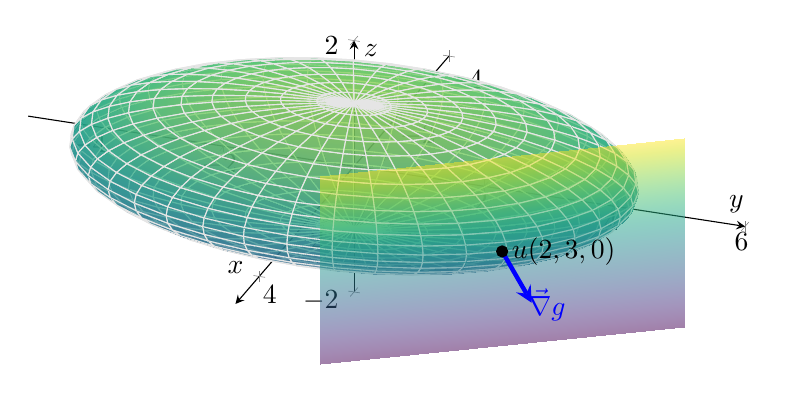
\begin{tikzpicture}
    \begin{axis}[
        axis lines = center,
        xlabel = $x$, ylabel = $y$, zlabel = $z$,
        view/h=110, view/v=25,    % Angle ajusté pour bien voir le point de contact
        colormap/viridis,
        z buffer=sort,
        xmin=-4, xmax=5,
        ymin=-5, ymax=6,
        zmin=-2, zmax=2,
        height=10cm, width=14cm,
        axis equal image          % Proportions réelles
    ]

    % --- 1. L'ELLIPSOÏDE ---
    \addplot3[
        surf,
        shader=faceted interp,
        fill opacity=0.7,
        faceted color=black!10,
        domain=0:360,
        domain y=0:180,
        samples=40, samples y=25,
        variable=u, variable y=v,
        point meta=z
    ]
    (
        {sqrt(8) * sin(v) * cos(u)},
        {sqrt(18) * sin(v) * sin(u)},
        {cos(v)}
    );

    % --- 2. LE PLAN TANGENT ---
    % Équation : x/2 + y/3 = 2  => y = 6 - 1.5x
    % C'est un plan vertical. Paramétrisation : x=t, y=6-1.5t, z=h
    \addplot3[
        surf,
        shader=interp,
        color=red,
        fill opacity=0.5,
        % On choisit un domaine autour de x=2 pour le plan
        domain=0.5:3.5,       % Variation de x (autour de 2)
        domain y=-1.5:1.5,    % Variation de z (hauteur du plan)
        samples=2,            % Plan plat, pas besoin de bcp de points
        variable=t,           % t joue le rôle de x
        variable y=h          % h joue le rôle de z
    ]
    (
        t,              % x
        {6 - 1.5*t},    % y
        h               % z
    );

    % --- 3. POINT DE CONTACT ET GRADIENT ---
    
    % Le point u(2, 3, 0)
    \addplot3[only marks, mark=*, mark size=2pt, color=black] coordinates {(2,3,0)};
    \node[right] at (axis cs:2,3,0) {$u(2,3,0)$};

    % Le vecteur gradient (1/2, 1/3, 0)
    % On l'agrandit (x3) pour qu'il soit visible, car 1/2 est petit par rapport aux axes
    \draw[->, blue, ultra thick, >=stealth] 
        (axis cs: 2, 3, 0) -- 
        (axis cs: {2 + 1.5}, {3 + 1}, 0) 
        node[midway, below right] {$\vec{\nabla}g$};

    \end{axis}
\end{tikzpicture}
\caption{Plan tangent à l'ellipsoïde en $u$}
\end{center}
\end{figure}

\begin{exemple}
    On pose $X$ l'ellipsoide d'équation $\displaystyle \frac{x^2} 8 + \frac{y^2}{18} + z^2 = 1$.

    Soit alors $u = (2, 3, 0) \in X$. 

    On a donc $X = g^{-1}(\{0\})$ avec 
    $$\fonction{g}{\R^3}{\R}{(x, y, z)}{\frac{x^2} 8 + \frac{y^2}{18} + z^2 - 1}$$
    et $g$ est $\mathscr C^1$ sur $\R^3$. 

    $\ds \grad g (x, y, z) = \left( \frac{x} 4, \frac{y} 9, 2z \right)$ en 
    $\ds u = (2, 3, 0)$, $\ds \grad g(u) = \left( \frac 1 2, \frac 1 3, 0 \right) \neq 0$.

    Donc $u$ est régulier et posons $P$ le plan affine tangent à $X$ en $u$.

    On a donc $(x, y, z) \in P$ ssi $(x, y, z) - u \in T_uX$ ssi $(x - 2, y - 3, z - 0) \perp \grad g(u)$ ssi
    $$\frac 1 2 (x - 2) + \frac 1 3 (y - 3) + 0 (z - 0) = 0$$

    Donc $M (x, y, z) \in P$ ssi $\displaystyle \frac x 2 + \frac y 3 = 2$.
\end{exemple}

\begin{figure}[h]
\begin{center}

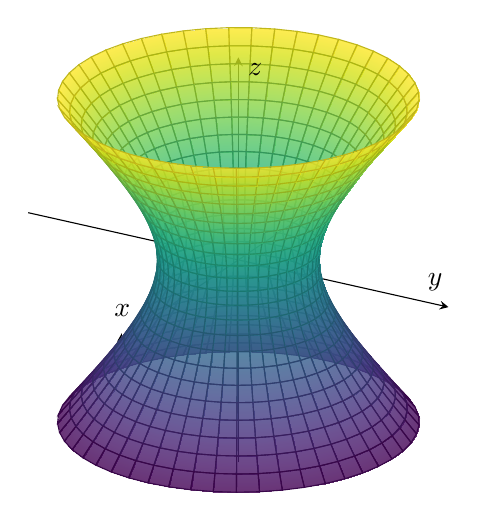
\begin{tikzpicture}
    \begin{axis}[
        axis lines = center,      % Axes au centre
        xlabel = $x$, ylabel = $y$, zlabel = $z$,
        ticks=none,               % Retire les chiffres pour un look épuré (optionnel)
        view/h=120,               % Angle de vue horizontal
        view/v=25,                % Angle de vue vertical
        colormap/viridis,         % Palette de couleurs
        z buffer=sort,            % ESSENTIEL pour que les faces cachées soient derrière
        xmin=-3, xmax=3,
        ymin=-3, ymax=3,
        zmin=-2.5, zmax=2.5,
        height=10cm, width=10cm   % Taille de la figure
    ]

    % Paramétrage de l'hyperboloïde à une nappe
    % x = sqrt(1+z^2) * cos(angle)
    % y = sqrt(1+z^2) * sin(angle)
    % z = z
    \addplot3[
        surf,                   % Surface
        shader=faceted interp,  % Lissage avec lignes de maillage légères
        fill opacity=0.8,       % Légère transparence
        domain=-2:2,            % Hauteur z (variable u)
        domain y=0:360,         % Angle de rotation (variable v)
        samples=25,             % Précision verticale
        samples y=50,           % Précision circulaire
        variable=u,             % u correspond à z
        variable y=v,           % v correspond à l'angle
        point meta=u            % La couleur dépend de la hauteur z
    ]
    (
        {sqrt(1+u^2)*cos(v)},   % x
        {sqrt(1+u^2)*sin(v)},   % y
        {u}                     % z
    );

    \end{axis}
\end{tikzpicture}
\end{center}
\caption{Hyperboloïde à une nappe d'équation $x^2 + y^2 - z^2 = 1$}
\end{figure}

\begin{exemple}
    Soit $X$ l'hyperboloide à une nappe d'équation $x^2 + y^2 - z^2 = 1$.

    Soit $u \in X$, $u = (x, y, z)$, et on a $X = g^{-1}(\{0\})$ avec 
    $$\fonction{g}{\R^3}{\R}{(x, y, z)}{x^2 + y^2 - z^2 - 1}$$
    et $g$ est $\mathscr C^1$ sur $\R^3$.

    $\grad g (u) = (2x, 2y, -2z) \neq 0$ car sinon $x = y = z = 0$ et $g(0, 0, 0) = -1 \neq 0$.

    Soit alors $P$ le plan tangent en $u$ à $X$. Alors 

    \begin{align}
        M(\alpha, \beta, \gamma) \in P & \Leftrightarrow M - u \in T_uX \\
        & \Leftrightarrow M - u \perp \grad g(u) \\
        & \Leftrightarrow \langle (\alpha - x, \beta - y, \gamma - z), (2x, 2y, -2z) \rangle = 0 \\
        & \Leftrightarrow 2x \alpha + 2y \beta - 2z \gamma = 2x^2 + 2y^2 - 2z^2 = 2 \\
        & \Leftrightarrow x \alpha + y \beta - z \gamma = 1
    \end{align}
\end{exemple}

Référence donnée par Quibel pour comprendre la géométrie : BD de Anselm Lanturlu de J P Petit, geometricon. 

\section{Applications de classe \texorpdfstring{$\mathscr C^k $}{Ck}} 

Soit $\Omega$ un ouvert de $E$, avec $E$ un $\R$-espace vectoriel de dimension $p$, 
et $F$ un $\R$-espace vectoriel de dimension $n$, avec $f : \Omega \to F$.

On choisit $B = (e_1, \ldots, e_p)$ base de $E$ et $C = (c_1, \ldots, c_n)$ base de $F$.

Pour $x \in E$, ces choix permettent d'identifier $x = (x_1, \ldots, x_p) \in \R^p$
et $f(x) = (f_1(x), \ldots, f_n(x)) \in \R^n$ avec $\forall x \in \Omega$, 
$f(x) = \sum_{i=1}^n f_i(x) c_i$.

\subsection{Dérivée partielles d'ordre \texorpdfstring{$k$}{k}}

\begin{proposition}{Dérivées partielles d'ordre k}{}
    On dit que $f$ admet des dérivées partielles d'ordre $k \geqslant 1$ si pour tous 
    $j_1, \dots, j_k \in \ninter{1}{p}$, les fonctions
    $$\pp{}{x_{j_1}} \left( \cdots \left( \pp{}{x_{j_{k - 1}}} \left( \pp{f}{x_{j_k}} \right) \right) \right)$$
    existent sur $\Omega$.

    Cette fonction sera alors notée :

    $$\frac{\partial^k f}{\partial x_{j_1} \partial x_{j_2} \cdots \partial x_{j_k}} = \partial_{j_1} \partial_{j_2} \dots \partial_{j_k} f$$
\end{proposition}

\begin{definition}{Classe $\mathscr C^k$}{}
    \index{Classe $\mathscr C^k$}
    Soit $f : \Omega \to F$. On dit que $f$ est de classe $\mathscr C^k$ sur $\Omega$ si 
    $f$ admet toutes ses dérivées partielles d'ordre $k$ et que ces fonctions sont continues 
    sur $\Omega$.
\end{definition}

\begin{exemple}
    Si $f$ est polynomiale en les coordonnées, elles est de classe $\mathscr C^k$ pour tout 
    $k$ par théorème d'opérations. 

    $\fonction f {\R^3}\R{(x, y, z)}{x^2 y z - x y^3 z^2}$ est de classe $\mathscr C^\infty$.

    Il y a $9$ dérivées partielles d'ordre $2$, et on a : 
    \begin{itemize}
        \item $\displaystyle \pp f x = 2 x y z - y^3 z^2$
        \item $\displaystyle \pp f y = x^2 z - 3 x y^2 z^2$
        \item $\displaystyle \pp f z = x^2 y - 2 x y^3 z$
    \end{itemize}

    et donc il vient : 

    \begin{itemize}
        \item $\displaystyle \frac{\partial^2 f}{\partial x^2} = 2 x z - 3 y^2 z^2$
        \item $\displaystyle \frac{\partial^2 f}{\partial y \partial x} = 2 x z - 3 y^2 z^2$
        \item $\displaystyle \frac{\partial^2 f}{\partial z \partial x} = 2 x y - 2 y^3 z$
    \end{itemize}
\end{exemple}

\subsection{Théorème de Schwarz}

\begin{theoreme}{De Schwarz}{}
    Soit $f \in \mathscr C^2(\Omega, F)$.

    Alors pour tous $i, j \in \ninter{1}{p}$, on a 
    $$\frac{\partial^2 f}{\partial x_i \partial x_j} = \frac{\partial^2 f}{\partial x_j \partial x_i}$$
\end{theoreme}

\begin{proof}
    Non exigible.
\end{proof}

\begin{corollaire}{généralisation théorème de Schwarz}{}
    Si $f$ est de classe $\mathscr C^k$, l'ordre dans lequel on effectue les dérivations 
    dans le calcul d'une dérivée partielle d'ordre $k$ n'a pas d'importance.
\end{corollaire}

\subsection{Opérations sur les fonctions de classe \texorpdfstring{$\mc k$}{Ck}}

\begin{proposition}{Opérations sur les applications de classe $\mathscr C^k$}{}
    Soient $f, g \in \mathscr C^k(\Omega, F)$ et $\alpha, \beta \in \R$, alors 
    $\alpha f + \beta g \in \mathscr C^k(\Omega, F)$ et pour tous 
    $j_1, \ldots, j_k \in \ninter{1}{p}$, on a :
    $$\frac{\partial^k (\alpha f + \beta g)}{\partial x_{j_1} \cdots \partial x_{j_k}} = \alpha \frac{\partial^k f}{\partial x_{j_1} \cdots \partial x_{j_k}} + \beta \frac{\partial^k g}{\partial x_{j_1} \cdots \partial x_{j_k}}$$
\end{proposition}

\begin{proof}
    Non exigible. 
\end{proof}

\begin{proposition}{Composition d'applications de classe $\mathscr C^k$}{}
    Une composée d'applications de classe $\mathscr C^k$ est de classe $\mathscr C^k$.
\end{proposition}

\begin{proof}
    Non exigible.
\end{proof}

\begin{exemple}
    Calcul du laplacien en polaires.

    Soit 
    $$\fonction \varphi {\R^2}{\R^2}{(r, \theta)}{\begin{pmatrix} 
        r \cos(\theta) \\
        r \sin (\theta)
    \end{pmatrix}}$$
    Alors $\varphi$ est $\mathscr C^2$ par théorème d'opérations, et 
    
    soit $\fonction f {\R^2}{\R}{(x, y)}{f(x, y)}$ de classe $\mathscr C^2$.

    \svspace Soit $F = f \circ \varphi : \R^2 \to \R$, $F(r, \theta) = f(r \cos(\theta), r \sin(\theta))$.

    Par composition, $F$ est de classe $\mathscr C^2$.

    \begin{align}
        \pp F r (r, \theta) & = \pp f r \begin{pmatrix}
        r \cos(\theta) \\
        r \sin(\theta)
    \end{pmatrix} \\
    & = \cos( \theta) \pp f x \begin{pmatrix}
        r \cos(\theta) \\
        r \sin(\theta)
    \end{pmatrix} + \sin(\theta) \pp f y \begin{pmatrix}
        r \cos(\theta) \\
        r \sin(\theta)
    \end{pmatrix}
    \end{align}

    \begin{align}
        \pp F \theta (r, \theta) & = \pp f \theta \begin{pmatrix}
        r \cos(\theta) \\
        r \sin(\theta)
    \end{pmatrix} \\
    & = - r \sin( \theta) \pp f x \begin{pmatrix}
        r \cos(\theta) \\
        r \sin(\theta)
    \end{pmatrix} + r \cos(\theta) \pp f y \begin{pmatrix}
        r \cos(\theta) \\
        r \sin(\theta)
    \end{pmatrix}
    \end{align} par la règle de la chaîne.

    En dérivant de nouveau, il vient :
    \begin{align}
        \frac{\partial^2 F}{\partial r^2} (r, \theta) & = \cos^2(\theta) \frac{\partial^2 f}{\partial x^2} \begin{pmatrix}
        r \cos(\theta) \\
        r \sin(\theta)
    \end{pmatrix} + 2 \cos(\theta) \sin(\theta) \frac{\partial^2 f}{\partial x \partial y} \begin{pmatrix}
        r \cos(\theta) \\
        r \sin(\theta)
    \end{pmatrix} + \sin^2(\theta) \frac{\partial^2 f}{\partial y^2} \begin{pmatrix}
        r \cos(\theta) \\
        r \sin(\theta)
    \end{pmatrix}
    \end{align}

    $$\frac{\partial^2 F}{\partial r \partial \theta} = - \sin(\theta) \frac{\partial f}{\partial x} + \cos(\theta) \frac{\partial f}{\partial y} - r \sin(\theta) \cos(\theta) \frac{\partial^2 f}{\partial x^2} + r \cos^2(\theta) \frac{\partial^2 f}{\partial x \partial y} + r \cos \theta \sin \theta \frac{\partial^2 f}{\partial y^2}$$


    $$\frac{\partial^2 F}{\partial \theta^2} = - r \cos(\theta) \frac{\partial f}{\partial x} - r \sin(\theta) \frac{\partial f}{\partial y} + r^2 \sin^2(\theta) \frac{\partial^2 f}{\partial x^2} - 2 r^2 \sin(\theta) \cos(\theta) \frac{\partial^2 f}{\partial x \partial y} + r^2 \cos^2(\theta) \frac{\partial^2 f}{\partial y^2}$$

    En combinant, on trouve :
    $$\Delta f = \frac{\partial^2 f}{\partial r^2} + \frac 1 {r^2} \frac{\partial^2 f}{\partial \theta^2} + \frac 1 r \frac{\partial f}{\partial r}$$

    \begin{remarque}
        Les notations de la formule du laplacien en polaires sont quelque peu abusives, et la formule
        correcte serait plutôt :
        $$\Delta f = \frac{\partial^2F }{\partial r^2} + \frac 1 {r^2} \frac{\partial^2 F}{\partial \theta^2} + \frac 1 r \frac{\partial F}{\partial r}$$
    \end{remarque}
\end{exemple}

\subsection{\'Equations aux dérivées partielles }

On appelle EDP (équation aux dérivées partielles) d'ordre $k$ une équation d'inconnue $f \in \mathscr C^k(\Omega, F)$
faisant intervenir $f$ et certaines de ses dérivées partielles. 

\begin{theoreme}{Fonction constante le long des y}{}
    Soit $\Omega$ un ouvert convexe de $\R^2$ et $f \in \mathscr C^1(\Omega, \R)$.
    Si $\pp f y = 0$ alors en notant $\alpha = \inf \{x \in \R, \exists y \in \R, (x, y) \in \Omega\}$
    et $\beta = \sup \{x \in \R, \exists y \in \R, (x, y) \in \Omega\}$, il existe
    $\varphi \in \mathscr C^1(]\alpha, \beta[, \R)$ telle que
    $$\forall (x, y) \in \Omega, \, f(x, y) = \varphi(x)$$
\end{theoreme}

\idee{Intégrale pour l'existence, puis composition pour la régularité.}

\begin{proof}
    $\blacktriangleright$ Montrons l'existence de $\varphi$.
    
    Soit $f \in \mathscr C^1(\R, \R)$ telle que $\pp f y = 0$.

    Soit $x \in ] \alpha, \beta [$ et $y_1 < y_2$ tels que $(x, y_1), (x, y_2) \in \Omega$.

    $$ f(x, y_2) - f(x, y_1) = \int_{y_1}^{y_2} \pp f y (x, y) dy = 0$$
    
    car $\Omega$ convexe donc le segment $[(x, y_1), (x, y_2)] \subset \Omega$.

    Donc $f(x, y)$ ne dépend pas de $y$, donc notons $\varphi(x)$ sa valeur. 

    On a défini $\varphi : ]\alpha, \beta[ \to \R$ telle que 
    $\forall (x, y) \in \Omega, f(x, y) = \varphi(x)$.

    \lvspace 

    \marginenote{Explication}{On ne prend pas un $y$ quelconque car on composerait alors une application 
    $\mc 1$ ($f$) avec une application non nécessairement $\mc 1$ (le choix d'un $y$ quelconque).}

    \lvspace \avspace

    $\blacktriangleright$ Montrons maintenant que $\varphi$ est de classe $\mathscr C^1$.

    Soit $[a, b] \subset ]\alpha, \beta[$. En particulier notons 
    $y_a, y_b$ tels que $(a, y_a), (b, y_b) \in \Omega$.

    Alors $[(a, y_a), (b, y_b)] \subset \Omega$, et pour $x \in [a, b]$, considérons 
    $$y(x) = y_a + \frac{x - a }{ b - a } (y_b - y_a) \in S$$ donc dans $\Omega$

    Donc $\varphi(x) = f(x, y(x))$ = $f\left(x, y_a + \frac{x - a }{ b - a } (y_b - y_a) \right)$.

    Donc $\varphi$ est $ \mathscr C^1$ sur tout segment $[a, b]$ par composition, et donc sur $]\alpha, \beta[$.
\end{proof}

\begin{exemple}
    Contre exemple si $\Omega$ n'est pas convexe, mais seulement connexe ou étoilé (ce qui est
    le cas de $\Omega$ ici). 

    Posons $\Omega = \R^2 \setminus \{ (x, 0), x \leqslant 0 \} $
    et $f : (x, y) \mapsto \begin{cases}
        x^2 & \text{ si } x < 0 \text{ et } y < 0 \\
        -x^2 & \text{ si } x < 0  \text{ et } y > 0 \\
        0 & \text{ si } x \geqslant 0 \text{ et } y \neq 0 
    \end{cases}$

    Alors $f$ est $\mathscr C^1$, $\displaystyle \pp f y = 0$ et pourtant il n'existe pas de 
    $\varphi : \R \to \R$ telle que $\forall (x, y) \in \Omega, f(x, y) = \varphi(x)$.

    \avspace Soit $a \in \Omega$ tel que $a = (0, \alpha)$ avec $\alpha > 0$. 

    $\displaystyle \frac{f(a +  t(0, 1)) - f(a)}{t } = 0 \to 0$
    Donc $\displaystyle \pp f y (a) = 0$ et donc $\pp f y$ continue en $a$. 

    $\displaystyle \frac{f(a +  t(1, 0)) - f(a)}{t } = \frac{-t^2}{t} = -t \to 0$
    Donc $\displaystyle \pp f x (a) = 0$ et donc $\pp f x$ continue en $a$.

    Donc $f$ est $\mathscr C^1$ sur $\Omega$.
\end{exemple}

\begin{exemple}
    On cherche $f \in \mathscr C^1(\R^2, \R)$ telle que 

    (E) : $\ds \pp f x (x, y) = x + 3 y$

    (E) $ \Leftrightarrow \ds \pp{} x \left( f(x, y) - \frac{x^2} 2 - 3 xy \right) = 0$

    $\R$ étant convexe, par le théorème on a : 

    (E) $ \Leftrightarrow \exists \varphi \in \mathscr C^1(\R, \R), \forall (x, y) \in \R^2, 
    f(x, y) - \frac{x^2} 2 - 3xy = \varphi(y)$. 
    Donc la solution générale de (E) est :
    $$f(x, y) = \frac{x^2} 2 + 3xy + \varphi(y)$$
\end{exemple}

\begin{exemple}
    Cherchons $f \in \mc 1 (\R^2, \R)$, telle que $3 \ds \pp f x - 5 \pp f y = x - 2 y$

    L'idée est de faire un changement de variables en posant $(x, y) = \varphi(u, v)$
    et poser $F = f \circ \varphi$, puis bien choisir $\varphi$ pour obtenir une 
    équation différentielle en $F$ que l'on sait résoudre. Généralement, il faut soit 
    passer en polaire, soit utiliser une application linéaire pour le changement de variables.

    \avspace Posons $\fonction \varphi {\R^2}{\R^2}{(u, v)}{\begin{pmatrix}
        x = \alpha u + \beta v \\
        y = \gamma u + \tau v 
    \end{pmatrix}}$.

    On choisira $\alpha, \beta, \gamma$ et $\tau$ plus tard de façon astucieuse.
    
    On a donc $F = f \circ \varphi $ et donc 
    $\forall (u, v) \in \R^2$, $F(u, v) = f \begin{pmatrix}
        \alpha u + \beta v \\
        \gamma u + \tau v
    \end{pmatrix}$
    et $f$ étant $\mc 1$, $F$ l'est également et 

    \svspace \begin{itemize}
        \item $\ds \pp F u = \alpha \pp f x \begin{pmatrix}
            \alpha u + \beta v \\
            \gamma u + \tau v
        \end{pmatrix} + \gamma \pp f y \begin{pmatrix}
            \alpha u + \beta v \\
            \gamma u + \tau v
        \end{pmatrix}$
        \item $\ds \pp F v = \beta \pp f x \begin{pmatrix}
            \alpha u + \beta v \\
            \gamma u + \tau v
        \end{pmatrix} + \tau \pp f y \begin{pmatrix}
            \alpha u + \beta v \\
            \gamma u + \tau v
        \end{pmatrix}$
    \end{itemize}

    \svspace Choisissons par exemple $\alpha = 3$, $\beta = 0$, $\gamma = -5$ et $\tau = 1$.

    \avspace Alors il vient $\forall (u, v) \in \R^2$ :

    $$\ds \pp F u (u, v) = 3 \pp f x \begin{pmatrix}
        3 u \\
        -5 u + v
    \end{pmatrix} - 5 \pp f y \begin{pmatrix}
        3 u \\
        -5 u + v
    \end{pmatrix}$$

    et $\varphi$ est bijective, donc (E) $\Leftrightarrow \forall (u, v) \in \R^2$
    $\ds \pp F u (u, v) = 3 u - 2 (-5 + v)$ et $\ds \pp{} u \left( F(u, v) - \frac \beta 2 u^2 + 2 uv \right) = 0$.

    $\R^2$ convexe, donc $\ds \Leftrightarrow \exists \psi \in \mc 1 (\R, \R), \forall (u, v) \in \R^2$,
    $\ds F(u, v) - \frac {13} 2 u^2 - 2uv + \psi(v)$. 

    $\Leftrightarrow \forall (x, y) \in \R^2$,
    $$\ds f(x, y) = \frac{-7}{18} x^2 - \frac 2 3 x y + \psi(\frac 5 3 x + y)$$
\end{exemple}



\begin{exemple}
    $\ds x \pp f x + y \pp f y (x, y) = x$ avec $(x, y) \in (\R^*_+)^2$ en posant 
    en posant $\begin{cases}
        x = r \cos \theta \\
        y = r \sin \theta
    \end{cases}$ et considérons 
    $$\fonction \varphi {\R^*_+ \times ]0, \frac \pi 2 [}{(\R_+^*)^2}{(r, \theta)}{\begin{pmatrix}
        r \cos \theta \\
        r \sin \theta
    \end{pmatrix}}$$
    
    Alors $\varphi$ est bijective et $\mathscr C^1$. 

    Posons $F = f \circ \varphi$ et donc $$\fonction F {\R^*_+ \times ]0, \frac \pi 2 [}{\R}{(r, \theta)}{F(r, \theta) = f\begin{pmatrix}
        r \cos \theta \\
        r \sin \theta
    \end{pmatrix}}$$

    Alors $f$ est $\mc 1$ donc $F$ aussi et donc : 

    $$\pp F r (r, \theta) = \cos( \theta) \pp f x \begin{pmatrix}
        r \cos \theta \\
        r \sin \theta
    \end{pmatrix} + \sin(\theta) \pp f y \begin{pmatrix}
        r \cos \theta \\
        r \sin \theta
    \end{pmatrix}$$ 

    et puisque $\varphi$ est bijective, (E) $\Leftrightarrow \forall (r, \theta) \in \R^*_+ \times ]0, \frac \pi 2 [$,
    $$r \cos \theta \pp f x \begin{pmatrix}
        r \cos \theta \\
        r \sin \theta
    \end{pmatrix} + r \sin \theta \pp f y \begin{pmatrix}
        r \cos \theta \\
        r \sin \theta
    \end{pmatrix} = r \cos \theta$$

    \begin{align}
        \Leftrightarrow \ds r \pp F r (r, \theta) = r \cos \theta \\
        \Leftrightarrow \ds \pp F r (r, \theta) = \cos \theta \\
        \Leftrightarrow \ds \pp {} r \left( F(r, \theta) - r \cos \theta \right) = 0 \\
        \Leftrightarrow \ds \exists \psi \in \mc 1 \left( ]0, \frac \pi 2 [, \R \right), \forall (r, \theta) \in \R^*_+ \times ]0, \frac \pi 2 [
    \end{align}

    $$F(r, \theta) = r \cos \theta + \psi(\theta)$$

    $\Leftrightarrow \forall (x, y) \in (\R^*_+)^2$,
    $$f(x, y) = x + \psi \left( \arctan \left( \frac y x \right) \right)$$

    $\Leftrightarrow \exists g \in \mc 1 (\R_+^*, \R), \forall (x, y) \in (\R^*_+)^2$,
    $$f(x, y) = x + g \left( \frac y x \right)$$
\end{exemple}

\begin{remarque}
    On a calculé les dérivées partielles de $F$ en fonction de celles de $f$ et on a 
    "eu de la chance". On peut aussi expliciter $\varphi\inv $ et exprimer les dérivées de $f$ 
    en fonction de celles de $F$ puis remplacer dans l'EDP. 
\end{remarque}

Dans l'exemple précédent, on a $\forall (r, \theta) \in \R_+^* \times ]0, \frac \pi 2 [$, 
$\begin{cases}
    x = r \cos \theta \\
    y = r \sin \theta
\end{cases}$ 

et donc $\forall (x, y) \in (\R_+^*)^2$, 
$\ds \begin{cases}
    r = \sqrt{x^2 + y^2} \\
    \ds \theta = \arctan \left( \frac y x \right)
\end{cases}$.

$$\ds f(x, y) = F\left(\sqrt{x^2 + y^2}, \arctan \left( \frac y x \right)\right)$$

donc 

\begin{align}
        \pp f x (x, y) & = \frac x {\sqrt{x^2 + y^2}} \pp F r \begin{pmatrix}
        \sqrt{x^2 + y^2} \\
        \arctan \left( \frac y x \right)
    \end{pmatrix} + \left( \frac y {x^2} \frac 1 {1 + \frac{y^2}{x^2}} \right) \pp F \theta \begin{pmatrix}
        \sqrt{x^2 + y^2} \\
        \arctan \left( \frac y x \right)
    \end{pmatrix} \\
    & = \frac x {\sqrt{x^2 + y^2}} \pp F r \begin{pmatrix}
        \sqrt{x^2 + y^2} \\
        \arctan \left( \frac y x \right)
    \end{pmatrix} - \frac y {x^2 + y^2} \pp F \theta \begin{pmatrix}
        \sqrt{x^2 + y^2} \\
        \arctan \left( \frac y x \right)
    \end{pmatrix}
\end{align}

Et donc 

\begin{align}
    \pp f y (x, y) & = \frac y {\sqrt{x^2 + y^2}} \pp F r + \frac 1 x \frac{1}{1 + \frac{x^2}{y^2}} \pp F \theta \\
    & = \frac y {\sqrt{x^2 + y^2}} \pp F r + \frac x {x^2 + y^2} \pp F \theta
\end{align}

(E) $ \Leftrightarrow \forall (x, y) \in (\R_+^*)^2$,
$$ \frac{x^2 }{\sqrt{x^2 + y^2}} \pp F r - \frac{xy}{x^2 + y^2} \pp F \theta + \frac{y^2}{\sqrt{x^2 + y^2}} \pp F r + \frac{xy}{x^2 + y^2} \pp F \theta = x$$

$$\Leftrightarrow \sqrt{x^2 + y^2} \frac F r = x$$

$$\Leftrightarrow \forall r, \theta, \, r \pp F r (r, \theta) = r \cos \theta$$


\section{Optimisation }

\begin{definition}{Maximums et minimums locaux}{}
    \index{Extremum local}
    Soit $\Omega \subset E$ ouvert, $f : \Omega \to \R$ et $a \in \Omega$.

    On dit que $f$ présente un maximum (resp minimum) local en $a$ si il existe $R > 0$ 
    tel que $\forall x \in B(a, R) \cap \Omega$, $f(x) \leqslant f(a)$ (resp. $f(x) \geqslant f(a)$).

    Dans ce cas on dira que $f$ possède un extremum local en $a$. 
\end{definition}

\begin{definition}{Maximum et minimum globaux}{}
    \index{Extremum global}
    On dit que $f$ présente un maximum global en $a$ ssi $\forall x \in \Omega$, $f(x) \leqslant f(a)$.

    De même pour le minimum global.
\end{definition}

\begin{definition}{Point critique}{}
    \index{Point critique}
    Soit $f$ différentiable de $\Omega$ dans $\R$ et $a \in \Omega$. On dit que $a$ est un point critique de $f$ ssi
    $df(a) = 0$ et donc ssi $\grad f(a) = 0$ ssi toutes les dérivées partielles de $f$ en $a$ sont nulles.
\end{definition}

\begin{theoreme}{Condition nécessaire d'optimalité}{}
    Soit $f : \Omega \to \mathbb R$ différentiable et $a \in \Omega$. 

    Si $f$ présente un extremum local en $a$, alors $a$ est un point critique de $f$.
\end{theoreme}

\begin{proof}
    Soit $a$ en lequel $f$ présente un maximum local. Soit $j \in \ninter 1 p$. 

    Pour $t$ proche de 0, $a + t e_j \in \Omega$ et donc l'application
    partielle $\fonction{}{]- \varepsilon, \varepsilon[}{\R}{t}{f(a + t e_j)}$ présente un maximum en $t = 0$, donc
    sa dérivée $\pp f {x_j} (a) = 0$.

    Donc $df(a) = 0$.
\end{proof}

Attention, la réciproque est fausse en général. On peut avoir un point col pour 
lequel $f$ présente un maximum selon une direction et un min selon l'autre. 


\begin{exemple}
    Voci un contre exemple de la réciproque. 

    $$\fonction{f}{\R^2}{\R}{(x, y)}{x^2 - y^2}$$
    
    On a $f$ qui est $\mc 1$ et 
    $\ds \pp f x = 2x$ et $\ds \pp f y = -2y$.

    Donc $a = (0, 0)$ est un point critique de $f$.

    Pourtant pour $u_n = \left( \frac 1 n, 0 \right)$, et donc $u_n \to a$, on a 
    $f(u_n) > f(a)$ donc pas de max local en $a$. Pour $v_n = \left( 0, \frac 1 n \right)$,
    $v_n \to a$ et $f(v_n) < f(a)$ donc pas de min local en $a$.
\end{exemple}


Soit $C$ un compact de $E$ et $f : C \to \R$ continue. Alors par le théorème des bornes atteintes, 
$f$ est bornée et atteint ses bornes, donc présente un max et un min global en des points de $C$. 

Par ailleurs, $\mathring C = \Omega$ est un ouvert. Si les extremums globaux sont atteints en un point 
de $\Omega$, ce point est un point citique. Donc 
\begin{enumerate}
    \item On étudie $f$ sur $\Fr(C)$ et on y trouve son max $M$ et son min $m$.
    \item On compare $M$ et $m$ en les valeurs de $f$ en les points critiques
\end{enumerate}

\begin{exemple}
\tikzset{every picture/.style={line width=0.75pt}} %set default line width to 0.75pt        

\begin{center}
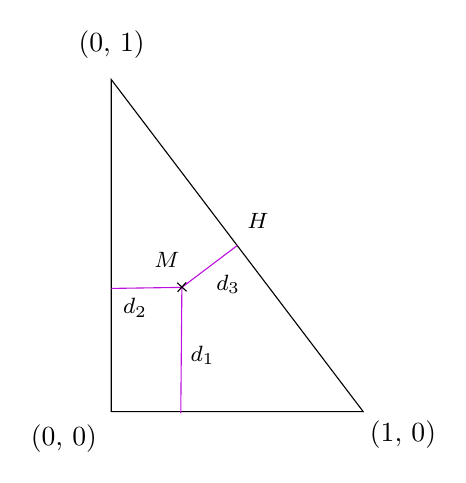
\begin{tikzpicture}[x=0.75pt,y=0.75pt,yscale=-1,xscale=1]
%uncomment if require: \path (0,300); %set diagram left start at 0, and has height of 300

%Shape: Right Triangle [id:dp4405477111777383] 
\draw   (256,71.71) -- (377.38,231.71) -- (256,231.71) -- cycle ;
%Straight Lines [id:da024450065100766527] 
\draw [color={rgb, 255:red, 189; green, 16; blue, 224 }  ,draw opacity=1 ]   (290.02,171.86) -- (289.5,232.5) ;
%Straight Lines [id:da2245066316000104] 
\draw [color={rgb, 255:red, 189; green, 16; blue, 224 }  ,draw opacity=1 ][fill={rgb, 255:red, 248; green, 231; blue, 28 }  ,fill opacity=1 ]   (256.02,172.36) -- (290.02,171.86) ;
%Straight Lines [id:da996469845251522] 
\draw [color={rgb, 255:red, 189; green, 16; blue, 224 }  ,draw opacity=1 ]   (316.69,151.71) -- (290.02,171.86) ;
\draw   (287.95,173.98) -- (292.14,169.41)(287.83,169.67) -- (292.26,173.73) ;

% Text Node
\draw (239,47) node [anchor=north west][inner sep=0.75pt]   [align=left] {(0, 1)};
% Text Node
\draw (216,237) node [anchor=north west][inner sep=0.75pt]   [align=left] {(0, 0)};
% Text Node
\draw (379.38,234.71) node [anchor=north west][inner sep=0.75pt]   [align=left] {(1, 0)};
% Text Node
\draw (293,199) node [anchor=north west][inner sep=0.75pt]  [font=\footnotesize] [align=left] {$\displaystyle d_{1}$};
% Text Node
\draw (260.5,176) node [anchor=north west][inner sep=0.75pt]  [font=\footnotesize] [align=left] {$\displaystyle d_{2}$};
% Text Node
\draw (305.36,164.79) node [anchor=north west][inner sep=0.75pt]  [font=\footnotesize] [align=left] {$\displaystyle d_{3}$};
% Text Node
\draw (275.5,153.5) node [anchor=north west][inner sep=0.75pt]  [font=\footnotesize] [align=left] {$\displaystyle M$};
% Text Node
\draw (320.3,134.7) node [anchor=north west][inner sep=0.75pt]  [font=\footnotesize] [align=left] {$\displaystyle H$};


\end{tikzpicture}
\end{center}
    \paragraph*{Preuve by Quibel :}
    $\fonction f T \R M {d_1 d_2 d_3}$. 

    $T$ est fermé borné donc compact. Sur le bord $\Fr(T), f= 0$ et sur $\mathring T$, $f > 0$. 
    Donc le min de $f$ est atteint en tout point de $\Fr(T)$. 

    $f$ est continue sur le compact $T$ Donc (bornes atteintes), le max de $f$ 
    existe. Comme $f$ est nulle sur la frontière, il est atteint en un point 
    d de $\mathring T$ qui est ouvert. 

    Pour $(x, y) \in T$, $f(x, y) = y x \frac{1 - (x + y)}{\sqrt 2}$. 

    L'hypothénuse a pour équation $x + y = 1$.

    $H(t, 1 - t)$ avec $t \in [0, 1]$ et $d^2(M, H) = d_3^2 = (t - x)^2 + (1 - t - y)^2 = g(t)$.
    
    Or en le projeté orthogonal, $g(t)$ est minimale donc $g'(t) = 0$.

    C'est à dire que $2 (t - x) - 2(1 - t - y) = 0$ donc 
    $t - x - 1 + t+ y = 0$ et donc $t = \frac{1 + x - y}{2}$.

    $g(t) = \frac 1 2 (1 - x - y)^2$. 

    Donc $d_3 = \frac{ 1 - x - y}{\sqrt 2 }$. 

    $f$ est donc différentiable donc le max de $f$ est atteint en un point critique. 

    \begin{itemize}
        \item $\ds \pp f x = \frac{y}{\sqrt 2} (1 - 2x - y)$
        \item $\ds \pp f y = \frac{x}{\sqrt 2} (1 - x - 2y)$
    \end{itemize}

    en ce point : $x + y = 1 -x = 1 - y$ et donc $x = y = \frac 1 3$.

    Donc max de $f$ en $M\left( \frac 1 3, \frac 1 3 \right)$

    \lvspace \paragraph*{Preuve by Gemini} :

    \uindent{1. Expression analytique de la fonction}

    \svspace Soit $M(x,y)$ un point du triangle $T$. Les équations des trois côtés sont :
    \begin{itemize}
        \item L'axe des abscisses ($y=0$). La distance est $d_1 = |y| = y$.
        \item L'axe des ordonnées ($x=0$). La distance est $d_2 = |x| = x$.
        \item L'hypoténuse reliant $(1,0)$ à $(0,1)$, d'équation cartésienne $x+y-1=0$.
    \end{itemize}

    La distance $d_3$ d'un point $M(x,y)$ à la droite d'équation $ax+by+c=0$ est donnée par la formule $\ds \frac{|ax+by+c|}{\sqrt{a^2+b^2}}$. Ici :
    \[
    d_3 = \frac{|x+y-1|}{\sqrt{1^2+1^2}} = \frac{1-x-y}{\sqrt{2}}
    \]
    (La valeur absolue est retirée car pour tout $M \in T$, $x+y \le 1$, donc $1-x-y \ge 0$).

    La fonction à étudier sur le domaine $T$ est donc :
    \[
    f(x,y) = x \cdot y \cdot \frac{1-x-y}{\sqrt{2}} = \frac{1}{\sqrt{2}} (xy - x^2y - xy^2)
    \]

    \uindent{2. Argument topologique (Existence et localisation)}

    \svspace \begin{itemize}
        \item L'ensemble $T$ est fermé et borné dans $\mathbb{R}^2$, c'est donc un \textbf{compact}.
        \item La fonction $f$ est polynomiale, donc continue sur $T$.
    \end{itemize}
    D'après le théorème des bornes atteintes, $f$ admet un maximum global sur $T$.

    Étudions le comportement au bord (frontière $\partial T$) et à l'intérieur (ouvert $\mathring{T}$) :
    \begin{itemize}
        \item Sur le bord $\partial T$, au moins une des distances ($x$, $y$ ou $1-x-y$) est nulle. Donc $f(x,y) = 0$ sur $\partial T$.
        \item À l'intérieur $\mathring{T}$, les distances sont strictement positives, donc $f(x,y) > 0$.
    \end{itemize}
    Par conséquent, le maximum ne peut pas être atteint sur le bord. Il est nécessairement atteint en un point de l'ouvert $\mathring{T}$.
    Puisque $f$ est différentiable sur l'ouvert $\mathring{T}$, ce maximum doit être un \textbf{point critique} (point où le gradient s'annule).

    \uindent{3. Calcul différentiel}

    \svspace Calculons les dérivées partielles de $f$ :
    \[
    \frac{\partial f}{\partial x} = \frac{1}{\sqrt{2}} (y - 2xy - y^2) = \frac{y}{\sqrt{2}} (1 - 2x - y)
    \]
    \[
    \frac{\partial f}{\partial y} = \frac{1}{\sqrt{2}} (x - x^2 - 2xy) = \frac{x}{\sqrt{2}} (1 - x - 2y)
    \]

    On cherche les points critiques $(x,y) \in \mathring{T}$, ce qui implique $x \neq 0$ et $y \neq 0$. L'annulation du gradient $\nabla f(x,y) = \vec{0}$ équivaut au système linéaire suivant :
    \[
    \begin{cases}
    1 - 2x - y = 0 \\
    1 - x - 2y = 0
    \end{cases}
    \]
    Par soustraction des deux lignes : $(-2x - y) - (-x - 2y) = 0 \implies -x + y = 0 \implies x = y$.

    En injectant $x=y$ dans la première équation :
    \[
    1 - 2x - x = 0 \implies 3x = 1 \implies x = \frac{1}{3}
    \]
    On obtient donc un unique point critique $M(\frac{1}{3}, \frac{1}{3})$.

    \uindent{Conclusion}

    \svspace Puisque le maximum existe et qu'il doit être un point critique intérieur, le maximum de $f$ est atteint au point de coordonnées $\ds \left(\frac{1}{3}, \frac{1}{3}\right)$.
\end{exemple}


\begin{remarque}
    Si $D : ax + by = c$, alors la distance de $M(x, y)$ à $D$ est 
    $\displaystyle d(M, D) = \frac{|ax + by - c|}{\sqrt{a^2 + b^2}}$.
\end{remarque}


\subsection{Optimisation sous contraintes}

\marginenote{Intuition}{On peut voir cela comme se promener sur un chemin à 
une altitude constante.}

\lvspace
\avspace

\begin{propositionnt}{condition nécessaire d'optimalité sous contraintes}{}
    Soit $\Omega$ ouvert de $E$ et $f : \Omega \to \R$. Soit $X \subset \Omega$ non vide, et 
    $x \in X$. 

    Si $f_{|_X}$ présente en $x$ un extremum local et si $f$ est différentiable en $x$ alors 
    pour tout $v \in T_xX$, $df(x)(v) = 0$, c'est à dire que $\grad f(x) \perp v$. 
\end{propositionnt}

\idee{
    Prendre un voisinage et composer avec un chemin, puis formule différentielle de la composition.
}

\begin{proof}
    Soit $v \in T_xX$. Alors il existe un chemin $\gamma : \; ]-\varepsilon, \varepsilon[ \to X$
    tel que $\gamma(0) = x$ et $\gamma'(0) = v$.

    Supposons par exemple que $f_{|_X}$ présente un maximum local en $x$.

    Alors il existe $V$ voisinage de $x$ tel que $\forall y \in X \cap V$, $f(y) \leqslant f(x)$.

    $\gamma$ étant continue, il existe $\eta > 0$ tel que $\forall t \in ]-\eta, \eta[$, $\gamma(t) \in X \cap V$.

    Donc $f(\gamma(t)) \leqslant f(\gamma(0))$.

    Ainsi, $f \circ \gamma : ]-\eta, \eta[ \to \R$ présente un maximum local en $t = 0$.
    Or $\gamma$ est dérivable en $0$, et $f$ est différentiable en $x$, donc 
    $f \circ \gamma$ est dérivable en $0$ et sa dérivée est nulle en $0$.

    Donc $df(\gamma(0))(\gamma'(0)) = 0$ et donc $df(x)(v) = 0$.
\end{proof}

\begin{theoreme}{D'optimisation sous contrainte}{}
    Soient $f, g \in \mc 1 (\Omega, \R)$ et posons $X = g^{-1}(0)$.
    Soit $x \in X$ tel que $dg(x) \neq 0$. 

    Si $f_{|_X}$ présente un extremum local en $x$ alors $df(x)$ est colinéaire à $dg(x)$. 

    En particulier, si $E$ est euclidien, $\grad f (x)$ est colinéaire à $\grad g(x)$.
\end{theoreme}

\begin{proof}
    En munissant $E$ d'une structure euclidienne. 

    Grâce à l'hypothèse, on a $T_x X = \ker (dg(x))$. 

    Par la proposition, $\underbrace{\ker (dg(x))}_{\text{hyperplan}} \subset \ker (df(x))$.

    Or $\Vect(\grad(g(x)))^\perp \subset \Vect(\grad (f(x)))^\perp$

    Donc $\Vect(\grad (f(x))) \subset \Vect(\grad (g(x)))$.

    Donc $\grad f(x)$ est colinéaire à $\grad g(x)$.
\end{proof}

\begin{proof}
    Autre preuve ne nécessitant pas de structure euclidienne.

    Supposons que $f_{|_X}$ admette un extremum local en $a \in X$ tel que $g(a) = 0$ et $dg(a) \neq 0$. Alors : 
    \begin{itemize}
        \item On a $T_a X = \ker(dg(a))$.
        \item Par la proposition précédente, $\ker(dg(a)) \subset \ker(df(a))$.
        \item Puisque $f$ et $g$ sont des fonctions numériques, $df(a)$ et $dg(a)$ sont des formes linéaires.
        \begin{itemize}
            \item Si $df(a) \neq 0$, puisque $\ker(dg(a)) \neq 0$ par hypothèse, ces deux formes linéaires ont même 
            noyau donc sont propostionnelles et il existe ainsi $\lambda \in \R$ tel que $df(a) = \lambda dg(a)$.
            \item Si $df(a) = 0$, alors $df(a)$ est colinéaire à $dg(a)$ pour $\lambda = 0$. 
        \end{itemize}
    \end{itemize}
\end{proof}

\begin{exemple}
    

\tikzset{every picture/.style={line width=0.75pt}} %set default line width to 0.75pt        

\begin{center}

\begin{tikzpicture}[x=0.75pt,y=0.75pt,yscale=-1,xscale=1]
%uncomment if require: \path (0,300); %set diagram left start at 0, and has height of 300

%Straight Lines [id:da7868483769051047] 
\draw    (401.38,99.71) -- (465.38,208.71) ;
%Straight Lines [id:da4259069082358726] 
\draw    (354.38,168.71) -- (419.19,129.36) ;

% Text Node
\draw (294,145) node [anchor=north west][inner sep=0.75pt]  [font=\footnotesize] [align=left] {$\displaystyle M\ ( x_{0} ,\ y_{0})$};
% Text Node
\draw (482,193) node [anchor=north west][inner sep=0.75pt]   [align=left] {$\displaystyle  \begin{array}{c}
D\\
ax\ +\ by\ =\ c
\end{array}$};
% Text Node
\draw (423,104) node [anchor=north west][inner sep=0.75pt]  [font=\small] [align=left] {$\displaystyle H$};


\end{tikzpicture}

\end{center}

On cherche le point $H(x, y) \in D$ tel que $ d^2(M, H) $ soit minimale, avec $M(x_0, y_0)$ fixé.

$X = D = g^{-1}(\{c\})$ avec $g(x, y) = ax + by$.

On pose $f(x, y) = (x - x_0)^2 + (y - y_0)^2$ et par le théorème d'optimisation sous contrainte,
$\grad f (x, y)$ et $\grad g(x, y)$ sont colinéaires.

Donc leur déterminant est nul, et donc : 
$$\begin{vmatrix}
    2(x - x_0) & a \\
    2(y - y_0) & b
\end{vmatrix} = 0 = b(x - x_0) - a (y - y_0)$$

On retrouve le fait que $\overrightarrow{MH}$ est colinéaire à $\begin{pmatrix}
    a \\
    b
\end{pmatrix}$ qui est normal à $D$.
\end{exemple}

\begin{exemple}
    

\tikzset{every picture/.style={line width=0.75pt}} %set default line width to 0.75pt        

\begin{center}

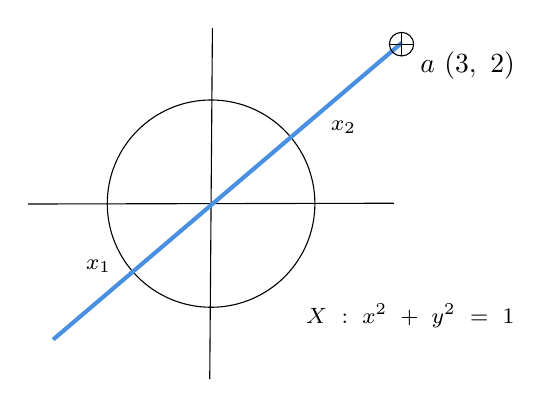
\begin{tikzpicture}[x=0.75pt,y=0.75pt,yscale=-1,xscale=1]
%uncomment if require: \path (0,300); %set diagram left start at 0, and has height of 300

%Straight Lines [id:da9773577401040182] 
\draw    (213.38,146.4) -- (389.57,146.03) ;
%Straight Lines [id:da3984499171199344] 
\draw    (302.12,61.71) -- (300.83,230.71) ;
%Shape: Ellipse [id:dp8119990119166796] 
\draw   (251.46,146.21) .. controls (251.46,118.64) and (273.85,96.28) .. (301.48,96.28) .. controls (329.1,96.28) and (351.49,118.64) .. (351.49,146.21) .. controls (351.49,173.79) and (329.1,196.15) .. (301.48,196.15) .. controls (273.85,196.15) and (251.46,173.79) .. (251.46,146.21) -- cycle ;
%Shape: Boxed Line [id:dp6810341271186268] 
\draw [color={rgb, 255:red, 74; green, 144; blue, 226 }  ,draw opacity=1 ][line width=1.5]    (225.38,211.71) -- (393.38,68.71) ;
%Flowchart: Or [id:dp962649201280356] 
\draw   (387.38,69.39) .. controls (387.38,66.26) and (390,63.71) .. (393.23,63.71) .. controls (396.45,63.71) and (399.07,66.26) .. (399.07,69.39) .. controls (399.07,72.53) and (396.45,75.07) .. (393.23,75.07) .. controls (390,75.07) and (387.38,72.53) .. (387.38,69.39) -- cycle ; \draw   (387.38,69.39) -- (399.07,69.39) ; \draw   (393.23,63.71) -- (393.23,75.07) ;

% Text Node
\draw (346,193) node [anchor=north west][inner sep=0.75pt]  [font=\footnotesize] [align=left] {$\displaystyle X\ :\ x^{2} \ +\ y^{2} \ =\ 1$};
% Text Node
\draw (240,172) node [anchor=north west][inner sep=0.75pt]  [font=\footnotesize] [align=left] {$\displaystyle x_{1}$};
% Text Node
\draw (358,105) node [anchor=north west][inner sep=0.75pt]  [font=\footnotesize] [align=left] {$\displaystyle x_{2}$};
% Text Node
\draw (401.07,71.71) node [anchor=north west][inner sep=0.75pt]   [align=left] {$\displaystyle a\ ( 3,\ 2)$};


\end{tikzpicture}

\end{center}

On cherche $ x \in X$ qui maximise $(x - 3)^2 + (y - 2)^2 = f(x, y) $. 

$f$ étant continue sur le compact $X$, il existe un point de $X$ en lequel $f$ est maximale (TBA). 

$g(x, y) = x^2 + y^2 - 1$ et $X = g^{-1}(\{0\})$. 

En le point $(x, y)$ recherché, $\grad f(x, y)$ et $\grad g(x, y)$ sont colinéaires.
Donc 

$$\begin{vmatrix}
    2(x - 3) & 2x \\
    2(y - 2) & 2y
\end{vmatrix} = 0$$

Donc $y(x - 3) - x(y - 2) = 0$ et donc $y = \frac 2 3 x$.
\end{exemple}

\begin{exemple}
    $A \in S_n(\R)$ et $u \in \R^n$ tel que $||u|| = 1$, c'est à dire que $u \in X = g\inv (\{0\})$ où 
    $g(u) = ||u||^2 - 1$.

    On pose $f(u) = \langle AU , U \rangle$ et $X$ est compact, $f$ est continue donc possède un max 
    et un min sur $X$. 

    En les vecteurs $U_1$ et $U_2$ en lesquels ce max et ce min sont atteints, on a 
    $\grad f(U)$ colinéaire à $\grad g(U)$. 

    On a $\forall H$, $dg(U)(H) = 2 \langle U , H \rangle = \langle 2 U , H \rangle$.

    Donc $\grad g (U) = 2 U \neq 0$. 

    Donc $U$ est régulier, et calculons $df(U)(H)$. 

    \begin{align}
        f(U + H) & = \langle A(U + H), U + H \rangle \\
        & = \langle AU, U \rangle + \langle AU, H \rangle + \langle AH, U \rangle + \langle AH, H \rangle \\
        & = f(U) + L(H) + ||H|| \varepsilon(H)
    \end{align}

    Avec $L(H) = \langle AU, H \rangle + \langle AH, U \rangle$ et $\varepsilon(H) = \ds \frac{\langle AH, H \rangle }{ || H||} \leqslant ||AH|| \to 0$

    Donc $f$ est différentiable et $df(U)(H) = \langle AU, H \rangle + \langle AH, U \rangle$
    Or 

    \begin{align}
        \langle AH, U \rangle & = (AH)^T u \\
        & = H^T A^T U \\
        & = H^T AU \\
        & = \langle H, AU \rangle 
    \end{align}

    Donc $df(U)(H) = 2 \langle AH, H \rangle$. 

    Donc $\grad f (U) = 2 AU$. Or en $U_i$, il est colinéaire à $\grad g (U_i)$ par 
    le théorème d'optimisation sous contrainte.Donc $\exists \alpha \in \R$, $2AU_i =  \alpha 2 U_i$

    Donc $U_i$ vecteur propre pour $A$ et $\alpha$ valeur propre. 
\end{exemple}


\subsection{\'Etude au second ordre}

\begin{definition}{Matrice hessienne}{}
    \index{Hessienne}
    Soit $\Omega \in \R^p$ et $B = (e_1, \ldots, e_p)$ une base orthonormée de $\R^p$
    telle que $\forall x \in \R^p$, $x = \ds \sum_{j = 1}^{p } x_j e_j$.

    Soit $f \in \mc 2(\Omega, \R)$ et $x \in \Omega$. On définit la matrice hessienne
    de $f$ en $x$ par : 
    $$H_f(x) = \left( \frac{\partial^2 f}{\partial x_i \partial x_j} (x) \right)_{1 \leqslant i, j \leqslant p}$$

    Grâce au théorème de Schwarz, $H_f(x)$ est symétrique.
\end{definition}

\begin{proposition}{Formule de Taylor-Young d'ordre 2}{}
    Soit $x \in \Omega$ et $h$ voisin de $0$ tel que $x + h \in \Omega$. Alors 
    $$f(x + h) = f(x) + \langle \grad f(x), h \rangle + \frac 1 2 \langle H_f(x) h, h \rangle + ||h||^2 \varepsilon(h) $$
\end{proposition}

\begin{remarque}
    On a $\langle H_f(x) h, h \rangle = \ds \sum_{i = 1 }^{p } (H_f(x) h)_i \cdot h_i = \sum_{i = 1}^{p } \left( \sum_{j = 1}^{p } \frac{\partial^2 f}{\partial x_i \partial x_j} (x) h_j \right) h_i$
\end{remarque}

\begin{proof}
    Non exigible. 
\end{proof}

\begin{definition}{Positivité et définie positivité d'une matrice symétrique}{}
    \index{Matrice!symétrique!positive}
    \index{Matrice!symétrique!definie positive@définie positive}
    Soit $S \in S_n(\R)$ matrice symétrique réelle. 
    \begin{itemize}
        \item On dit que $S$ est positive ssi $\Sp (S) \subset \R^+$. On note alors $S \in S_n^+(\R)$. 
        \item On dit que $S$ est définie positive ssi $\Sp(S) \subset \R_+^*$. On note alors $S \in S_n^{++}(\R)$.
    \end{itemize}
\end{definition}

\begin{theoreme}{Condition nécessaire d'extremum local au second ordre}{}
    Soit $f \in \mc 2 (\Omega, \R)$ et $x \in \Omega$. Si $f$ possède un minimum local
    (resp max local) en $x$ alors : 
    \begin{itemize}
        \item $\grad f (x) = 0$
        \item $H_f(x) \in S_n^+(\R)$ (resp $-H_f(x) \in S_n^+(\R)$) 
    \end{itemize}
\end{theoreme}

\idee{
    Absurde et DL en un vecteur propre. 
}

\begin{proof}
    Soit $x$ point critique de $f$. Soit $h$ un vecteur propre de 
    $H_f(x)$ pour une valeur propre $\lambda < 0$. 

    Soit $t \in \R$ voisin de $0$.

    $$f(x + th) = f(x) + \underbrace{df(x)(th)}_{= 0} + \frac 1 2 \langle H_f(x) (th), th \rangle + ||th||^2 \varepsilon(th)$$
    
    \begin{align}
        f(a + th) - f(x) & = \frac{1} 2 \langle \lambda th, th \rangle + t^2 ||h||^2 \varepsilon(th) \\
        & = \left( \frac \lambda 2 + \varepsilon(th) \right) t^2 ||h||^2 \\
        & < 0
    \end{align}

    qui est du signe de $\lambda$ quand $t$ tend vers $0$, car $\varepsilon(th) \to 0$.

    Donc $f$ n'a pas de minimum local en $x$ (resp maximum local).
\end{proof}

\begin{theoreme}{Condition suffisante d'extremum local au second ordre}{}
    Soit $f \in \mc 2 (\Omega, \R)$ et $x \in \Omega$. Si 
    \begin{itemize}
        \item $\grad f(x) = 0$
        \item $H_f(x) \in S_n^{++}(\R)$ 
    \end{itemize}
    alors $f$ possède un minimum local en $x$.
\end{theoreme}

\begin{remarque}
    Même délire avec le maximum local.
\end{remarque}

\begin{proof}
    Soit $f \in \mc 2 (\Omega, \R)$ et $x \in \Omega$ un point 
    critique tel que $H_f(x) \in S_n^{++}(\R)$.

    Par le théorème spectral, on peut choisir $B$ une base orthonormée de $\R^p$
    de vecteurs propres de $H_f(x)$. Notons $B = (e_1, \ldots, e_p)$ et
    $x = \ds \sum_{j = 1 }^{p } x_j e_j$.
    Donc 
    $$H_f(x) = \begin{pmatrix}
        \lambda_1 & 0 & \ldots & 0 \\
        0 & \lambda_2 & \ldots & 0 \\
        \vdots & \vdots & \ddots & \vdots \\
        0 & 0 & \ldots & \lambda_p
    \end{pmatrix}$$

    Soit $h$ proche de $0$, $h = \ds \sum_{j = 1}^{p } h_j e_j$.

    $$f(x + h) = f(x) + df(x)(h) + \frac 1 2 \langle H_f(x) h, h \rangle + ||h||^2 \varepsilon(h)$$

    et donc 

    $$f(x + h) - f(x) = \sum_{j = 1}^{p } \lambda_j h_j^2 + ||h||^2 \varepsilon(h)$$


    Notons $\alpha = \min(\lambda_1, \ldots, \lambda_p) > 0$.

    \begin{align}
        f(x + h) - f(x) & \geqslant \frac 1 2 \sum_{j = 1 }^{p } \alpha h_j^2 + ||h||^2 \varepsilon(h) \\
        & \geqslant \frac 1 2 \underbrace{\alpha + 2 \varepsilon(h)}_{\to \alpha > 0} ||h||^2
    \end{align}

    Donc on a un min local strict en $x$.
\end{proof}

\begin{proposition}{Cas particulier $p=2$}{}
    Soit $f : \Omega \to \R$ avec $\Omega \subset \R^2$ et 
    $a = \begin{pmatrix}
        x \\
        y
    \end{pmatrix} \in \Omega$ point critique de $f$.

    On note : 
    \begin{itemize}
        \item $\ds p = \pp f x (x, y)$
        \item $\ds q = \pp f y (x, y)$
        \item $\ds r = \ppn 2 f x (x, y)$
        \item $\ds s = \frac{\partial^2 f}{\partial x \partial y} (x, y)$
        \item $\ds t = \ppn 2 f y (x, y)$
    \end{itemize}

    En un point critique, $p = q = 0$ et $H_f(a) = \begin{pmatrix}
        r & s \\
        s & t
    \end{pmatrix}$.

    Notons $\lambda_1$ et $\lambda_2$ ses valeurs propres réelles. 

    $\lambda_1 \lambda_2 = rt - s^2= \det (H_f(a))$ et : 

    \begin{itemize}
        \item Si $rt - s^2 < 0$ alors $f$ n'a pas d'extremum local en $a$.
        \item Si $rt - s^2 > 0$ il y a un extremum local en $a$ :
        \begin{itemize}
            \item Si $r + t > 0$ alors $\lambda_1 + \lambda_2 > 0$, donc $\lambda_1 > 0$ et $\lambda_2 > 0$ donc $H_f(a) \in S_n^{++}(\R)$ et min local en $a$.
            \item Si $r + t < 0$ alors max local en $a$.
        \end{itemize}
    \end{itemize}
\end{proposition}